\section{Felhasználói dokumentáció}
Ez a fejezet tartalmazza a segítséget a regisztráció illetve bejelentkezés folyamatának sikeres végrehajtásához. A felhasználói műveletek alapvetően két csoportra bonthatóak:
\begin{itemize}
\item Azok a műveletek, amiket a felhasználó a telefonjának böngészőjében hajt végre
\item És a telefonra telepített bejelentkezést segítő android alkalmazás kezelése
\end{itemize}

Egy sikeres bejelentkezéshez ennek megfelelően futnia kell egy weboldalnak amely, előre definiált módon csatlakozik az E-Group IDX felhasználó-hitelesítési és azonosítási termékéhez.
A szakdolgozat keretein belül egy AngularJS weboldalt JavaEE (Spring keretrendszer) backend réteggel hoztunk létre és integráltuk a bejelentkezést a Spring Security rendszerébe.

\subsection{Mobil eszköz minimum követelményei}
A rendszer működése többnyire egy LG G3 telefonnal volt tesztelve, gyors és megbízható eredmények így a következő követelmények teljesülése esetén garantálhatóak.
\begin{itemize}
\item Minimum SDK 21-es verzió (Lollipop), Android 5.0
\item Minimum 2GB RAM
\item Quad-core 2.5 GHz Krait 400 CPU vagy erősebb
\item Előlapi kamera
\item NFC támogatottság
\end{itemize}

Természetesen ennél gyengébb eszközökön is fut az alkalmazás amennyiben minimum a 16-os SDK szintet (Jelly Bean) elér, és rendelkezik előlapi kamerával, ám a teljesítmény drasztikusan csökkenhet, szélsőséges esetben a bejelentkezéshez szükséges képtranszformációk sem kerülnek végrehajtásra, így a folyamat megszakadhat és a kérés elutasításra kerülhet.

\subsection{Mobil alkalmazás telepítése}
A mobil alkalmazás telepítését a telepítendő apk fájl birtokában azt megnyitva lehet elkezdeni. A műveletsor elején az android rendszer hozzáférést kér képkészítéshez, és NFC kommunikációhoz, ezek nélkül a telepítés nem tud folytatódni mivel elengedhetetlenek az alkalmazás megfelelő működéséhez (13. ábra).
\\Miután minden komponens települt azt egy sikeres telepítést jelző felirat jelzi (14. ábra).
\begin{figure}[h]
 \begin{minipage}{.5\textwidth} 
\centering
    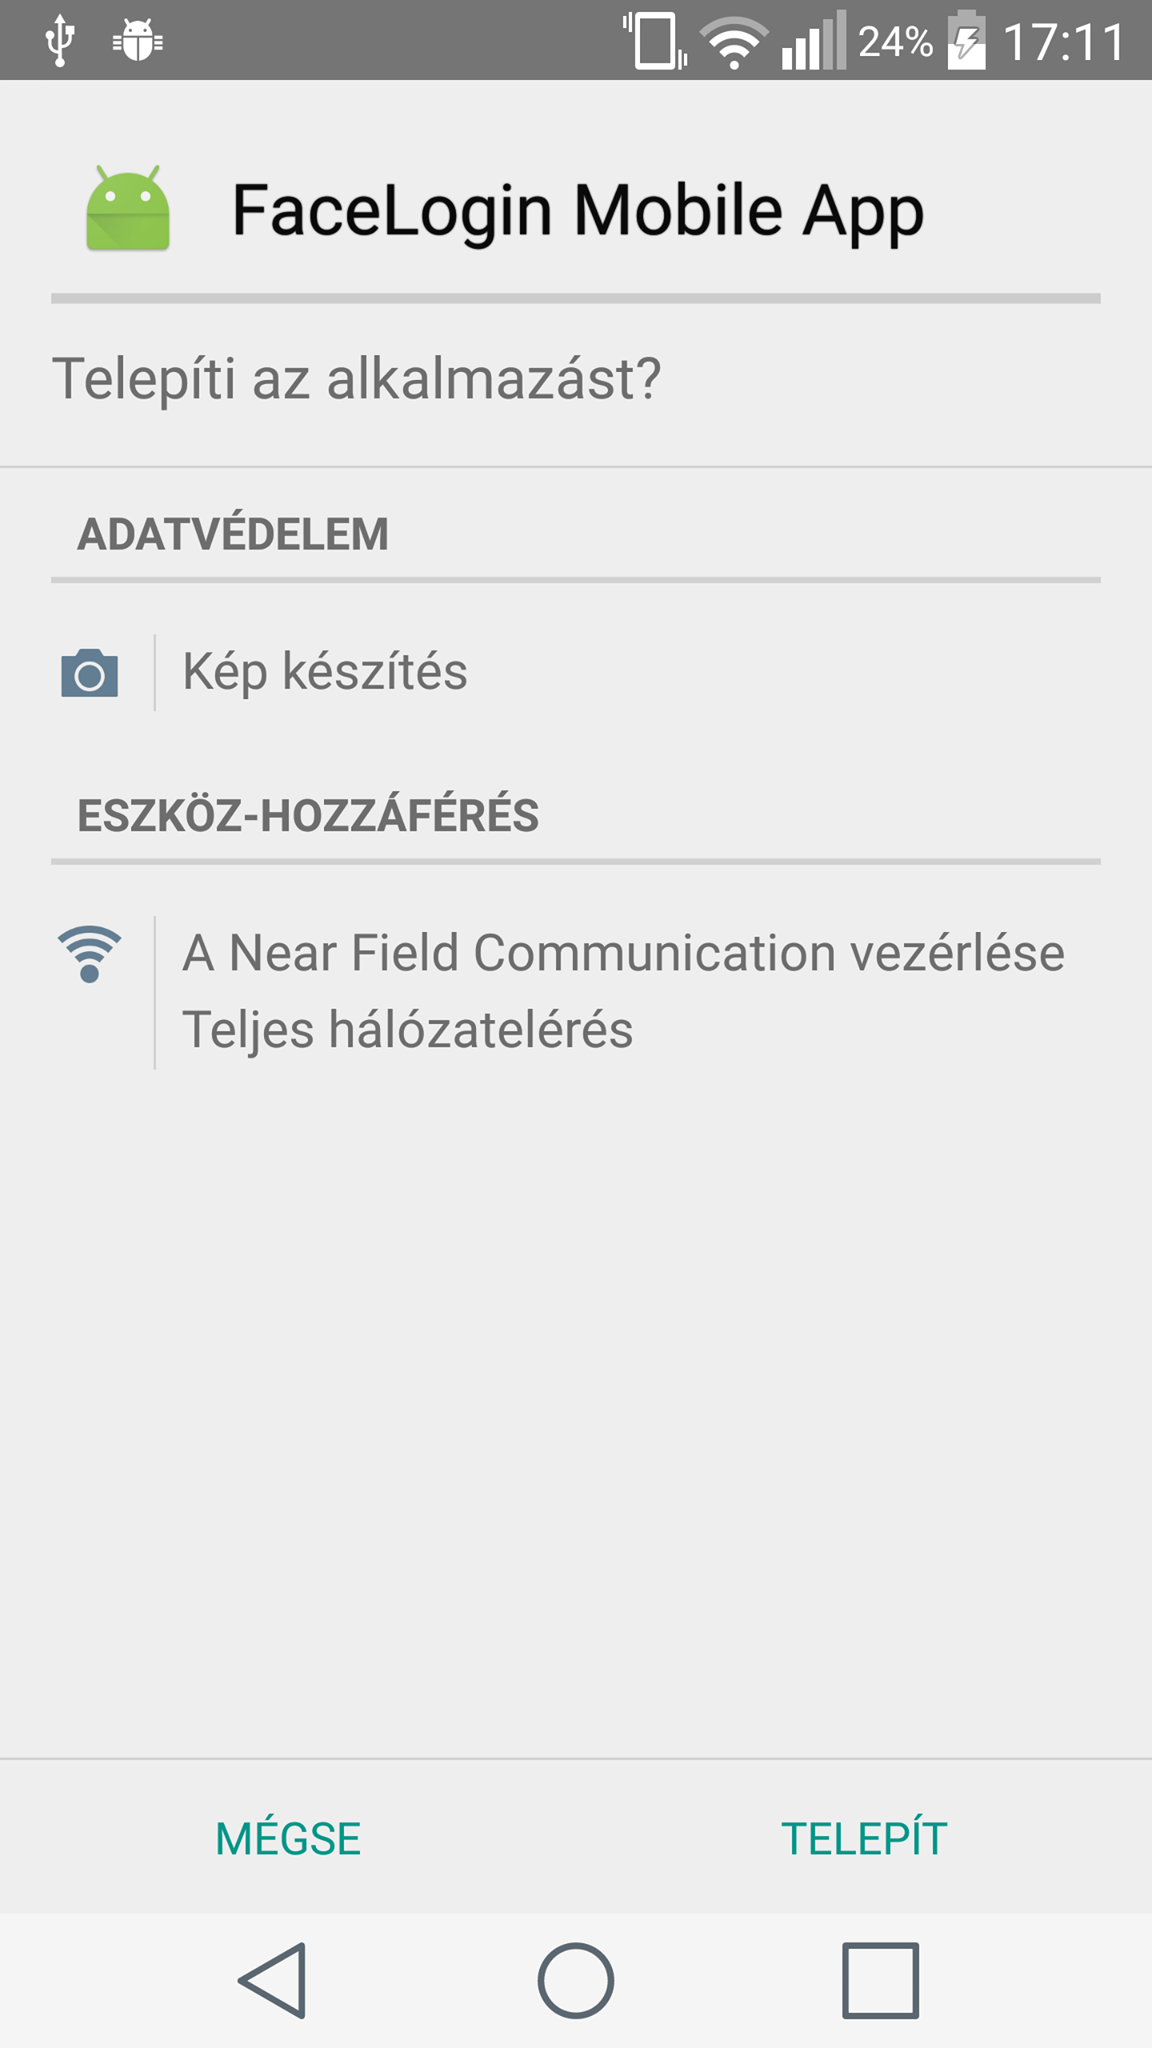
\includegraphics[scale=0.10]{img/install_app}
    \caption{Hozzáférések kérése}
 \end{minipage}
 \begin{minipage}{.5\textwidth} 
\centering
     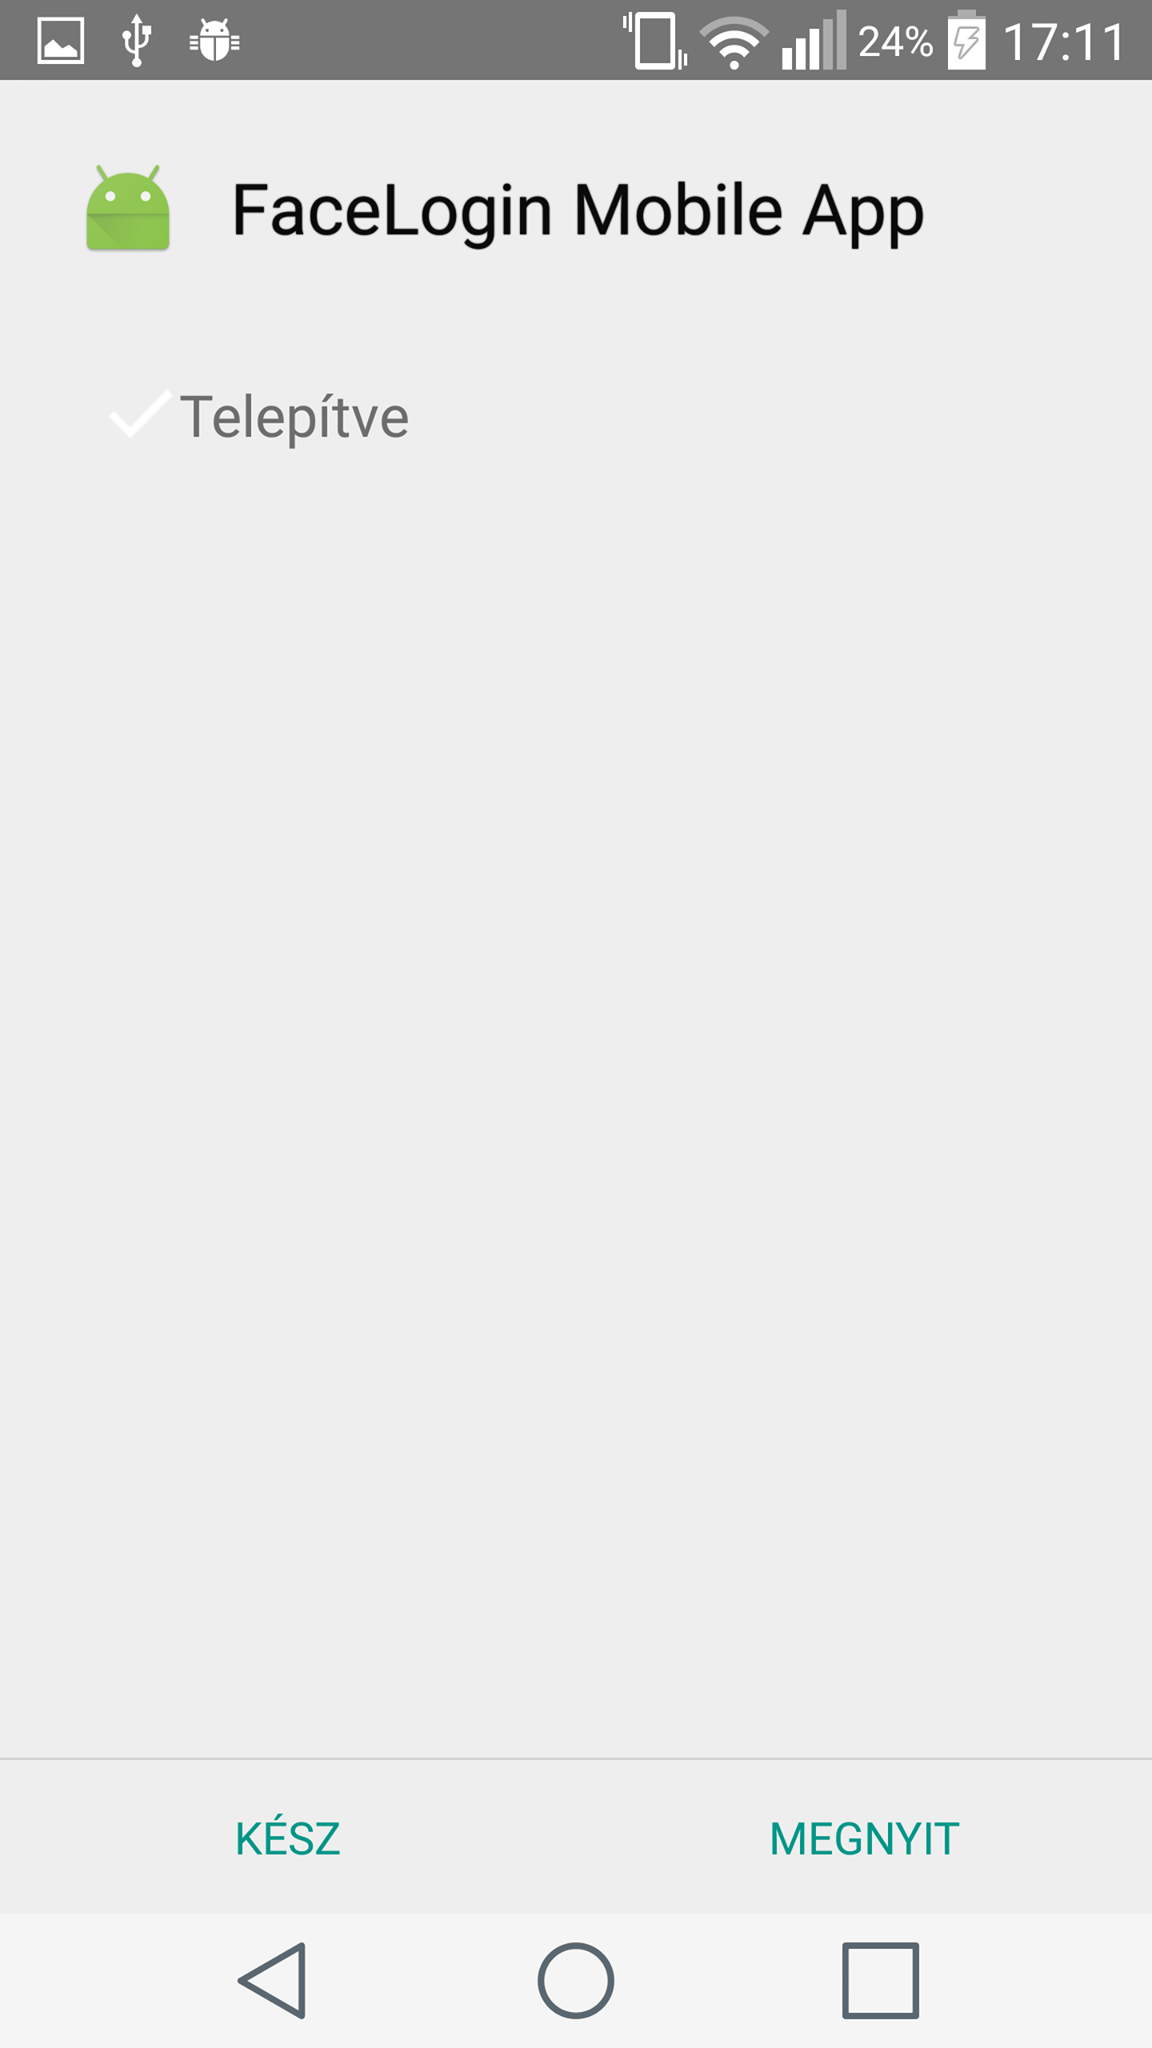
\includegraphics[scale=0.10]{img/app_installed}
     \caption{Telepítés sikeres}
 \end{minipage}
\end{figure}

\subsection{A webalkalmazás követelményei}
Az egyetlen követelmény hogy csatlakozzon  E-Group IDX felhasználó-hitelesítési és azonosítási termékének egy olyan verziójához, amiben megtalálható már a szakdolgozat keretében elkészített modul. Az integrálás módjáról a fejlesztői dokumentációban lehet olvasni.

\subsection{Az authentikáló alkalmazás követelményei}

Ez a modul egy Wildfly 10.1.0 verziójú szerveren fut, Java 8-as verzió alatt. Az indítási paraméterek között szerepel a
\begin{verbatim}
-Xms64m -Xmx512m 
\end{verbatim}
bejegyzés amely a minimum illetve a maximum allokálandó memóriát szabja meg. Ekkora memóriaterületen a rendszer működése megbízható, így ez minimum követelménynek tekinthető.


\subsection{Mobil alkalmazás figyelmeztető illetve hibaüzenetei}
Ez a fejezet a mobil alkalmazás lehetséges üzeneteit mutatja be, és leírást ad a lehetséges okokra. Nézzük először a főoldal üzeneteit, amik még azelőtt történnek, hogy a kártyát regisztráció vagy bejelentkezés céljából a telefonhoz tartanánk.
\begin{itemize}
\item Az alkalmazás valószínűleg nem jó időben lett megnyitva (nem egy felületről való kattintással inicializálta magát). Az alkalmazást így nem lehet használni, ezt üzenet jelzi a képernyő közepén (15. ábra). Amennyiben mégis megpróbáljuk elindítani az NFC olvasást, hibaüzenet jelenik meg
\item Nincsen minden kártyainformáció kitöltve (16. ábra). Ebben az esetben a jobb alsó sarokban található ceruza jelre kattintva megnyílik egy felület az adatok felvitelére. (17. ábra)
A kártyaszám megadásánál fontos a kisbetűk és nagybetűk megkülönböztetése. A két dátum megadásánál az alapértelmezett Android naptár komponens nyílik meg.
\item NFC ki van kapcsolva. Ez esetben bal alsó sarokban található csillagra kattintva a telefon megnyitja a beépített beállításkezelőt, ahol be lehet kapcsolni az NFC-t. A vissza gombra kattintva a folyamat innen tovább folytatható (18. ábra).
\end{itemize}

\begin{figure}[h]
 \begin{minipage}{.50\textwidth} 
\centering
    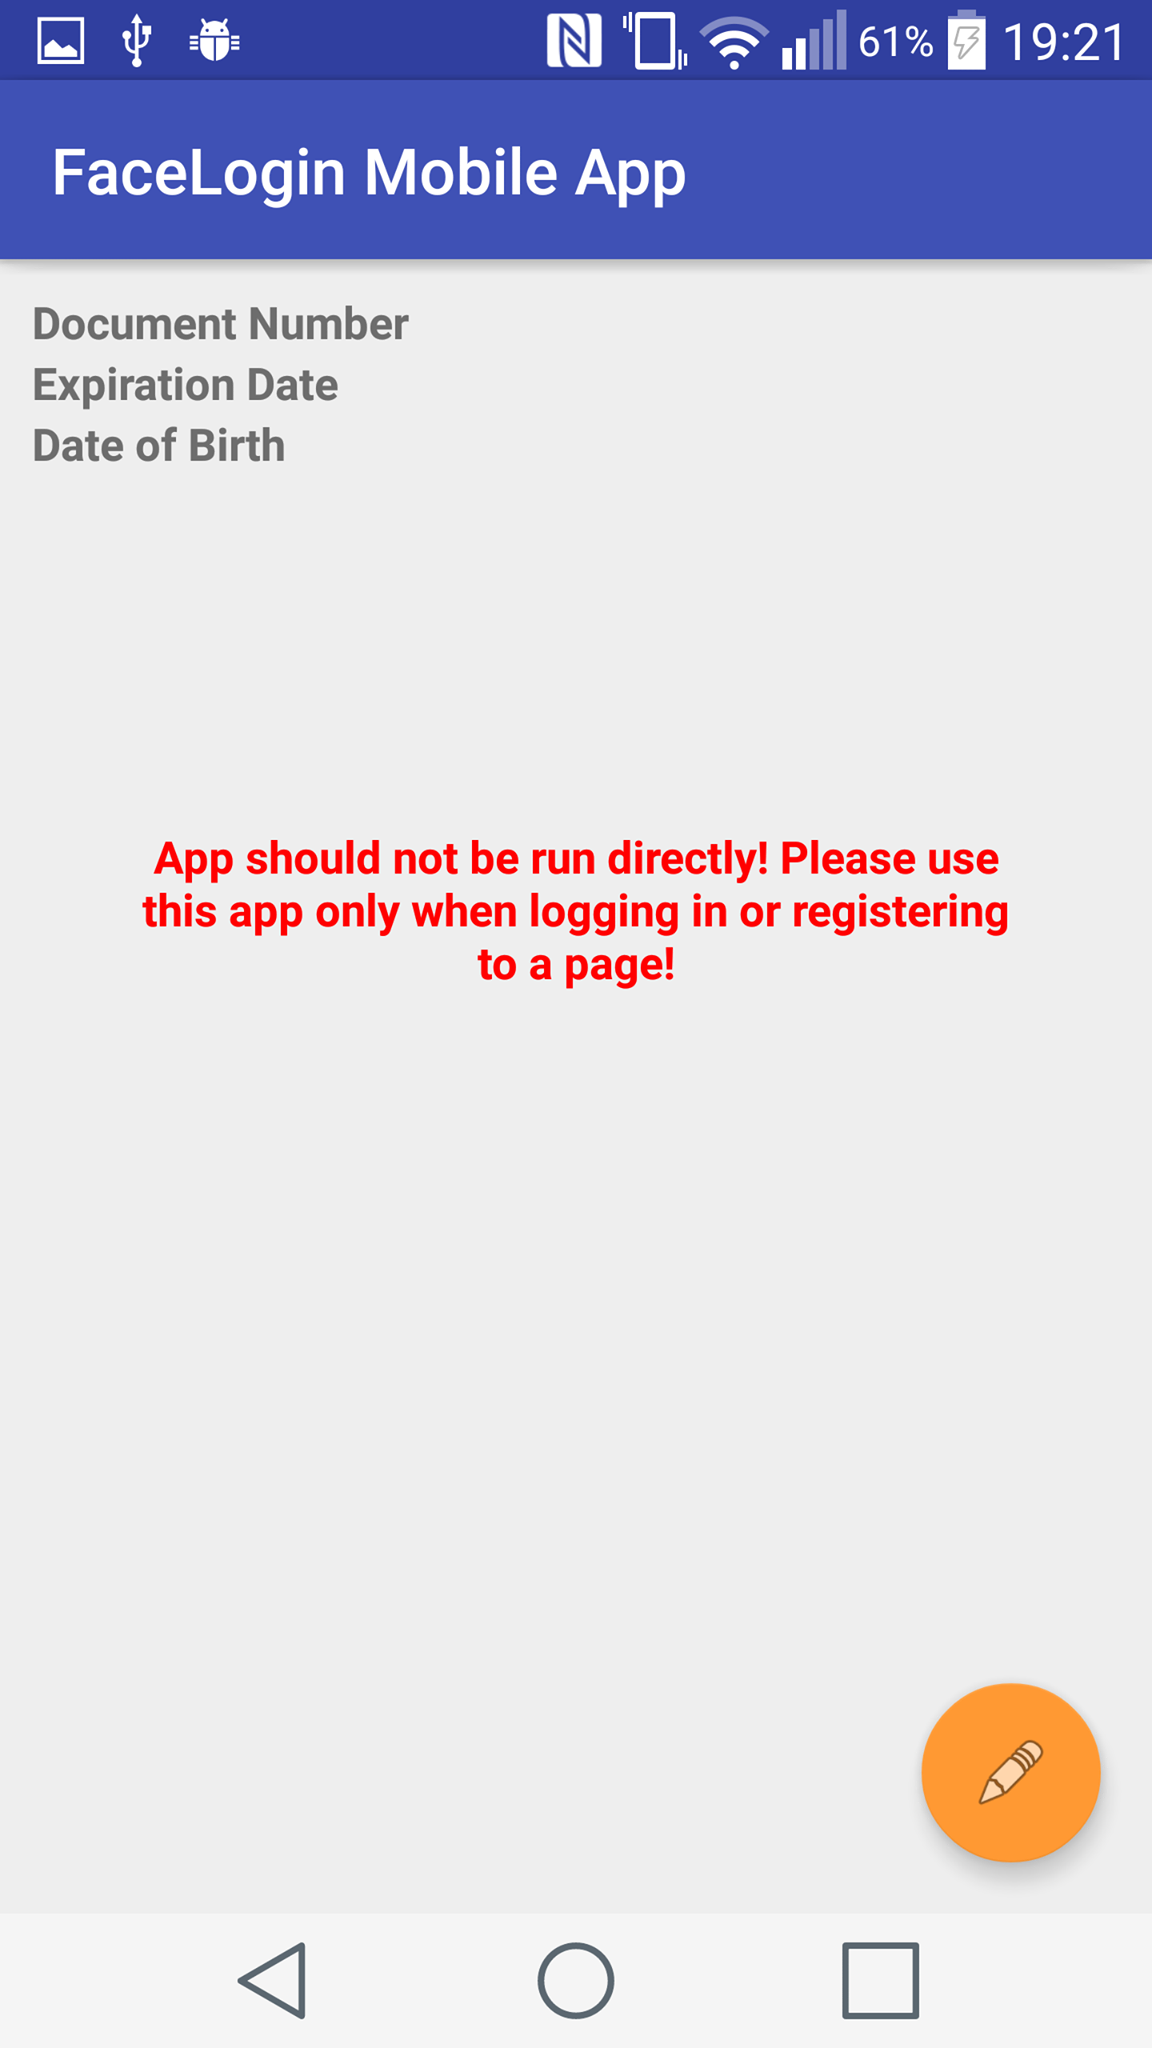
\includegraphics[scale=0.07]{img/app_should_not_be_run_directly}
    \caption{Alkalmazás csak felületről indítva futtatható}
 \end{minipage}
 \begin{minipage}{.50\textwidth} 
\centering
    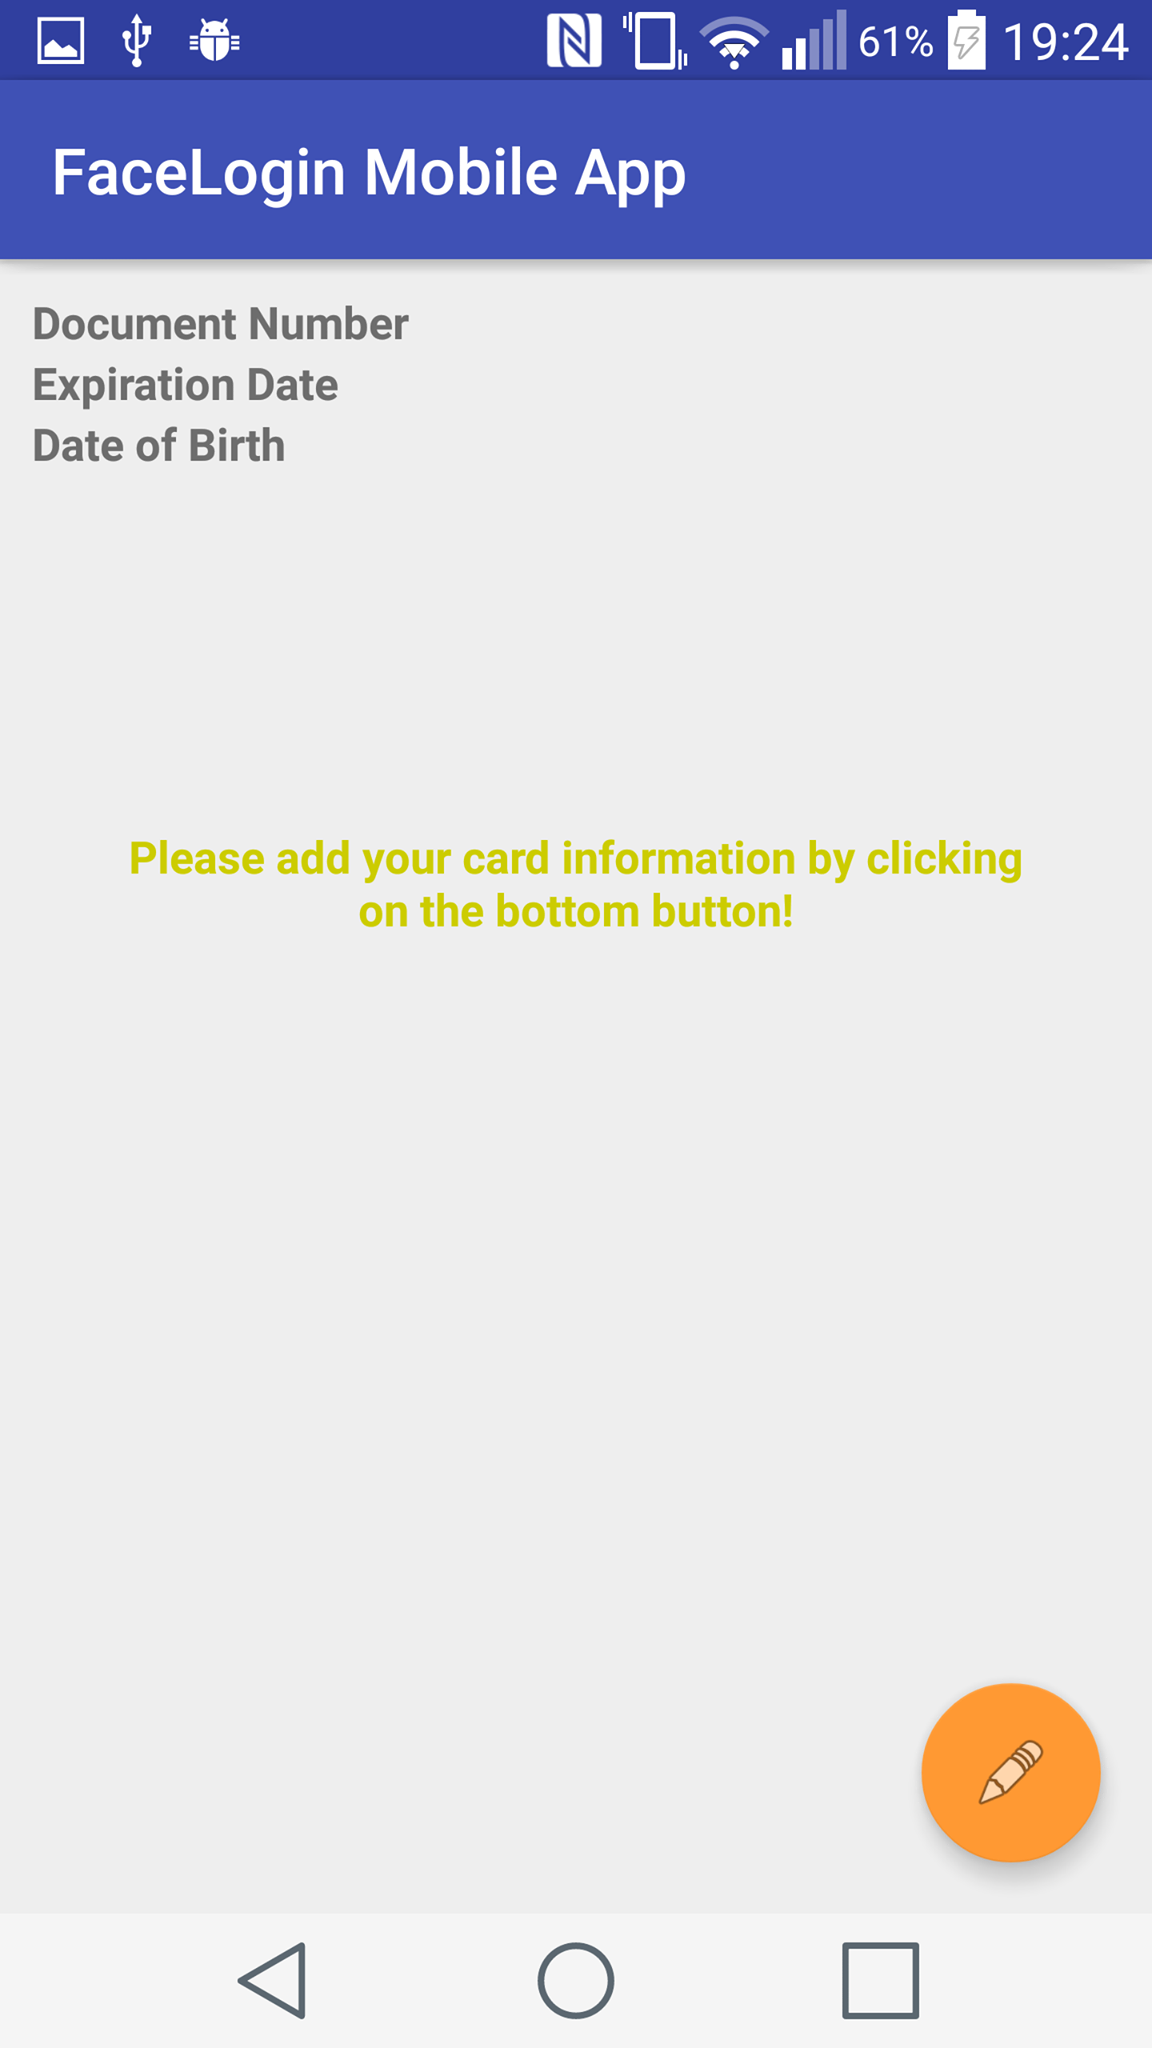
\includegraphics[scale=0.07]{img/not_enough_mrtd_data}
    \caption{Nincs minden adat kitöltve}
 \end{minipage}

 \begin{minipage}{.50\textwidth} 
\centering
    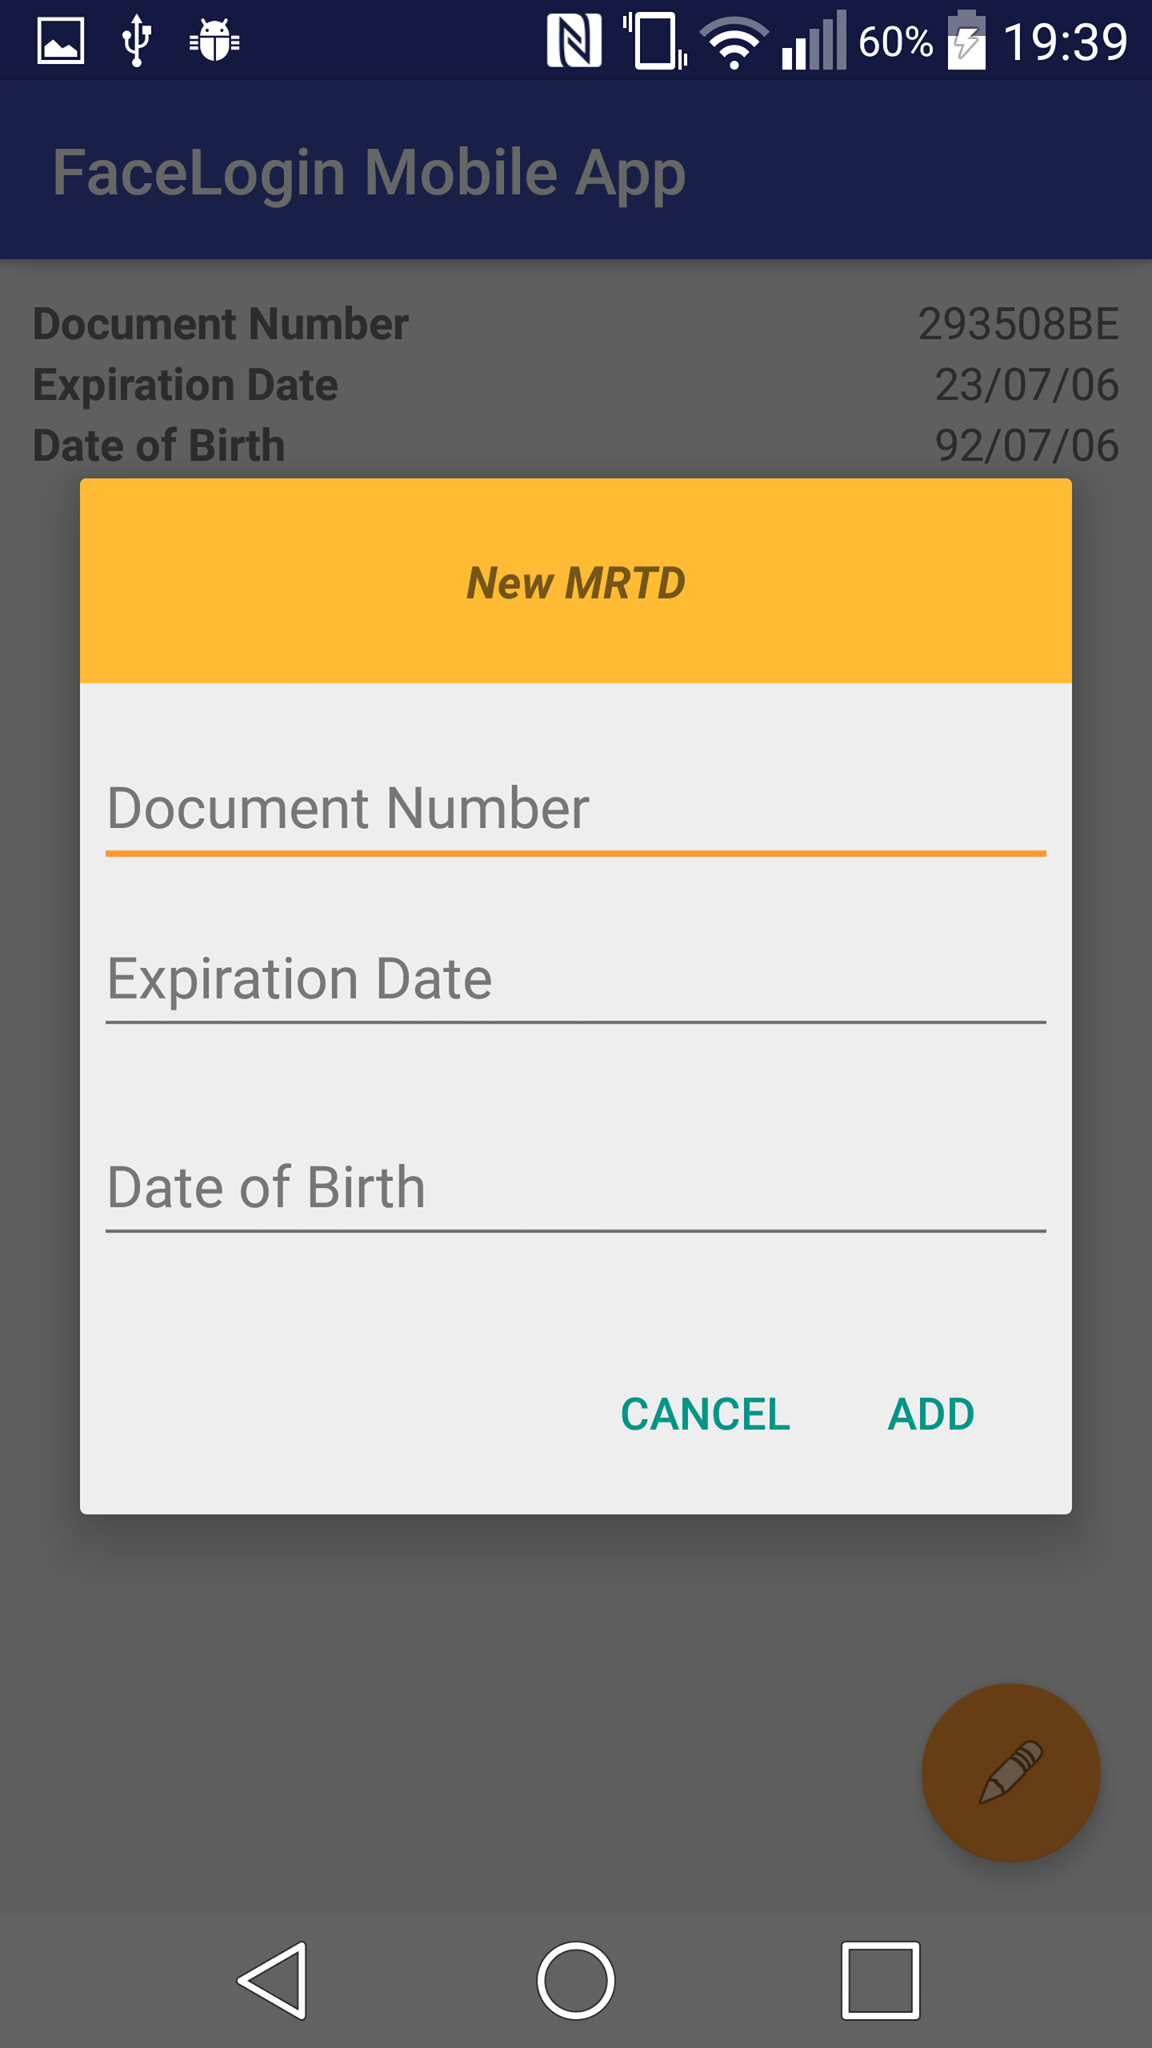
\includegraphics[scale=0.07]{img/new_mrtd}
    \caption{Új kártyaadatok felvitele}
 \end{minipage}
 \begin{minipage}{.50\textwidth} 
\centering
    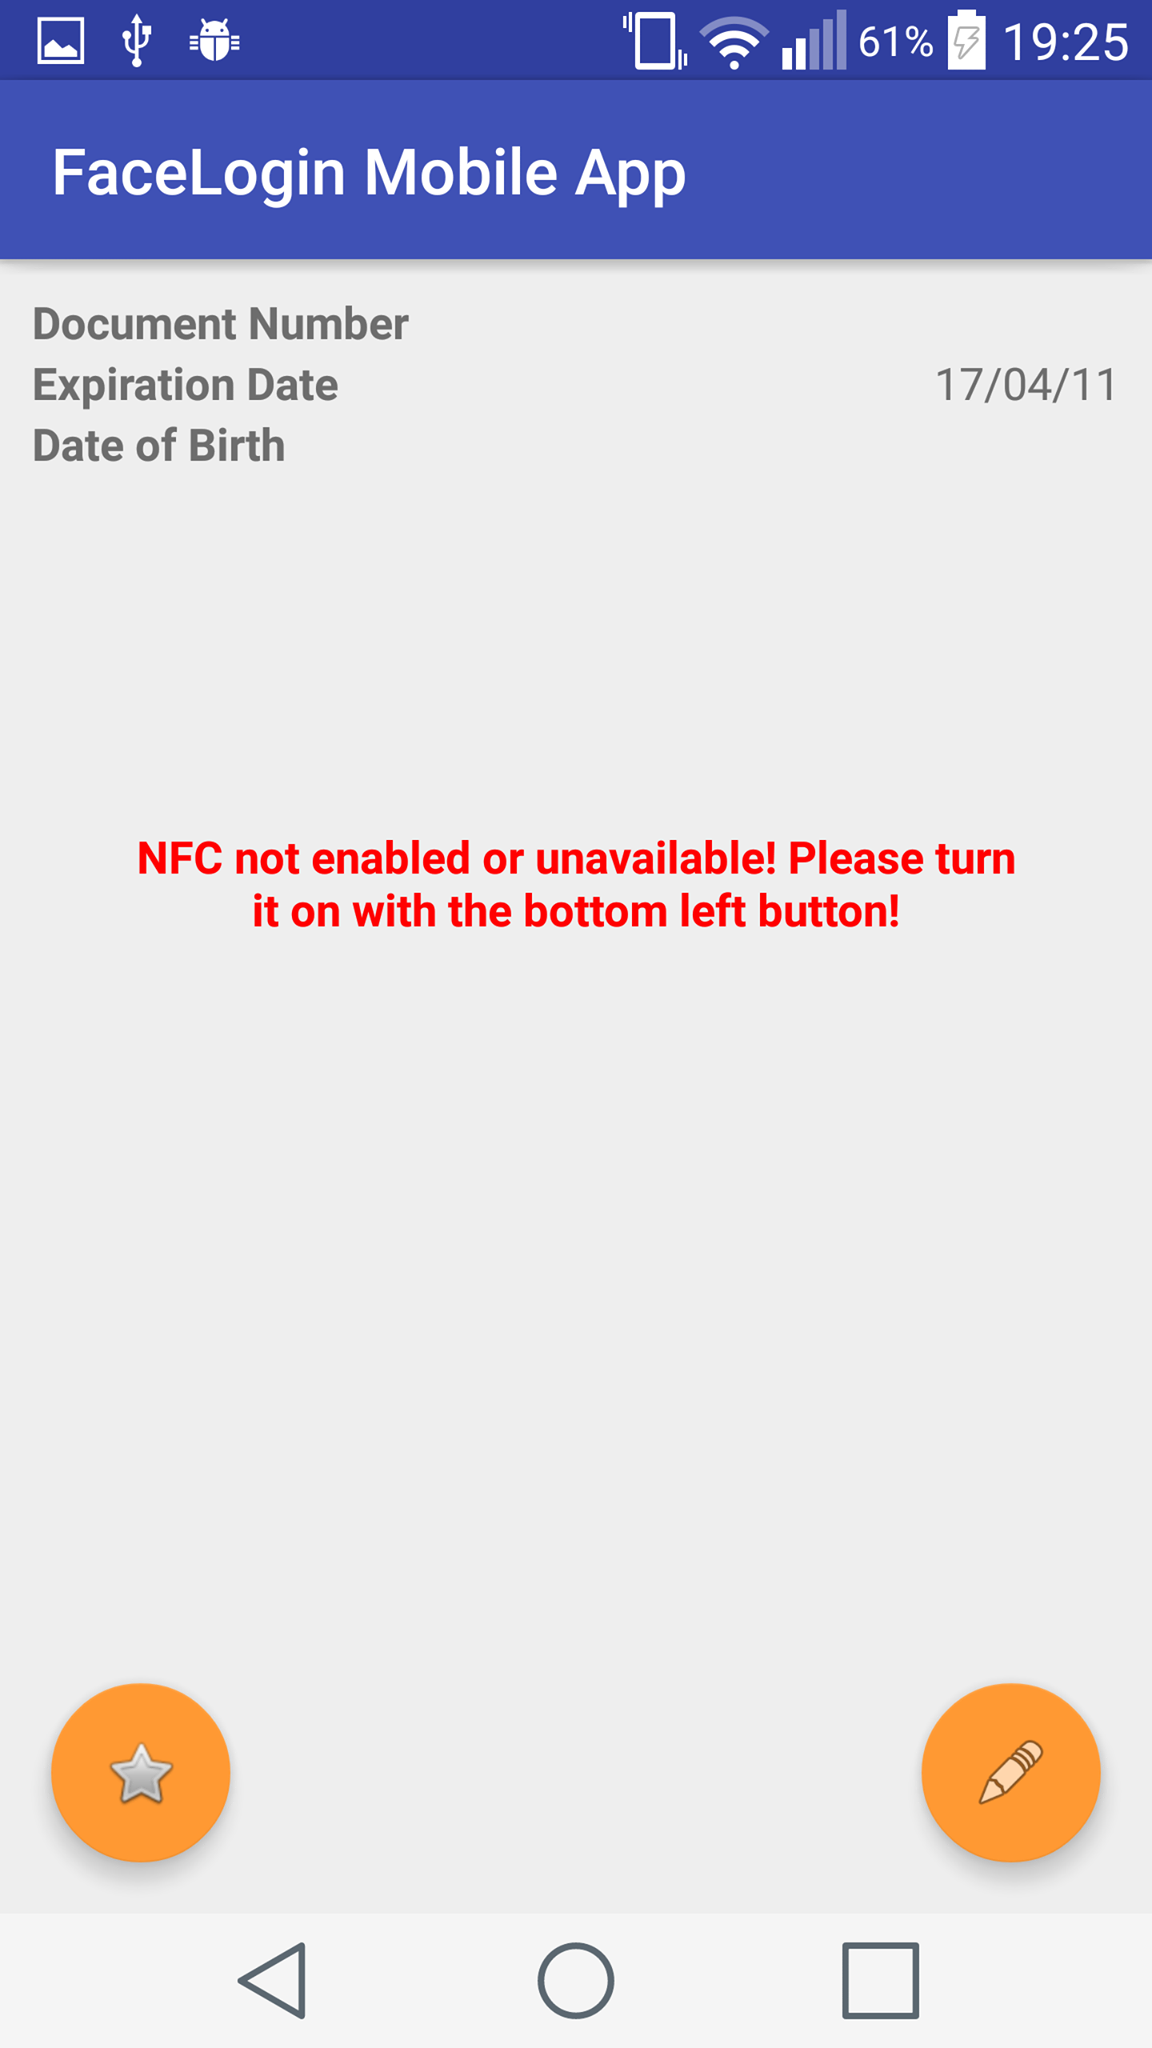
\includegraphics[scale=0.07]{img/nfc_not_enabled}
    \caption{NFC nincsen engedélyezve}
 \end{minipage}
\end{figure}

\clearpage
\subsection{A regisztráció folyamata}
A regisztráció folyamatát a rendszer működéséhez készített demonstrációs weboldalon keresztül mutatom be. Fontos megjegyezni, hogy akármilyen honlapra a weboldal technológiájától függően gyorsan vagy nehezebben, de integrálható a bejelentkezési modul, amennyiben az IDX szerveren be van állítva, hogy fogadja a kéréseket az adott címről.
\\A folyamat végrehajtásához az egész műveletsor Android mobiltelefonról kell, hogy végrehajtódjon, személyi számítógépről az alkalmazás nem fog megnyílni, és így nem lehetséges bejelentkezni!
\\Az oldal megnyitását követően a publikus főoldal látható. A regisztrációs oldalra való jutáshoz a "Sign Up" feliratra kell kattintani a bejelentkezés doboz alatt (19. ábra). A linkre kattintva megjelenik a regisztrációs felület (20. ábra). A szövegmezőbe kattintva adhatjuk meg a felhasználónevünket, majd a "START REGISTRATION" gombra kattintva indíthatjuk a regisztrációs folyamatot. Hibalehetőségek, amik esetén a műveletet megszakítja a rendszer és lehetőséget ad új felhasználónév megadására:
\begin{itemize}
\item A megadott felhasználónév már létezik a rendszerben (22. ábra)
\item Nincsen megadva felhasználónév (23. ábra)
\end{itemize}

Amennyiben a megadott név szabad, úgy egy új gomb jelenik meg "OPEN APP" felirattal (21. ábra). 
Erre a gombra kattintva a már feltelepített alkalmazás megnyílik, és a további információkat szolgáltatja.

\begin{figure}[h]
 \begin{minipage}{.30\textwidth} 
\centering
    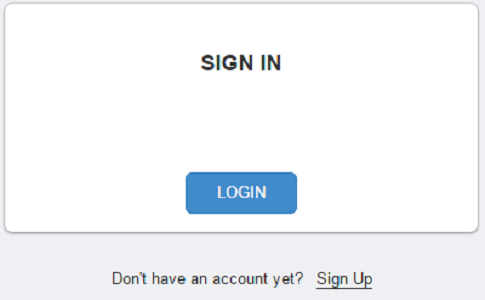
\includegraphics[scale=0.30]{img/sign_up_link}
    \caption{Publikus főoldal}
 \end{minipage}
 \begin{minipage}{.30\textwidth} 
\centering
     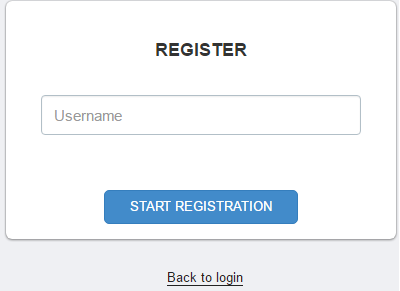
\includegraphics[scale=0.30]{img/register_page}
     \caption{Regisztrációs oldal}
 \end{minipage}
 \begin{minipage}{.30\textwidth} 
\centering
     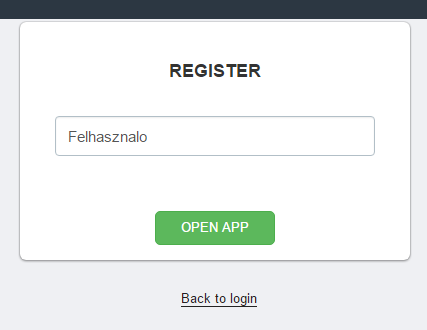
\includegraphics[scale=0.30]{img/open_app_registration}
     \caption{Alkalmazás megnyitása}
 \end{minipage}
\end{figure}

\begin{figure}[h]
 \begin{minipage}{.50\textwidth} 
\centering
    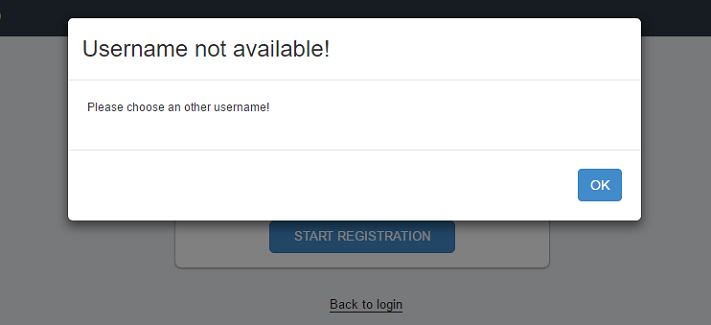
\includegraphics[scale=0.40]{img/username_not_available}
    \caption{Felhasználónév foglalt}
 \end{minipage}
 \begin{minipage}{.50\textwidth} 
\centering
     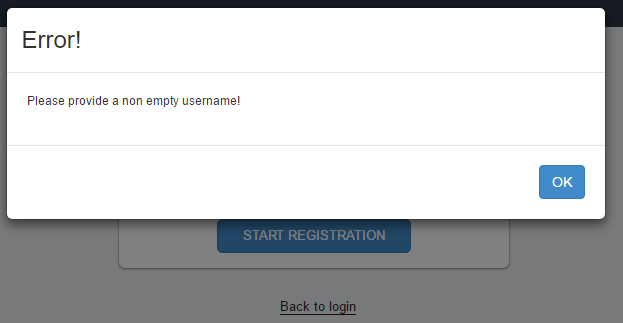
\includegraphics[scale=0.40]{img/username_empty}
     \caption{Nincsen megadva felhasználónév}
 \end{minipage}
\end{figure}
\clearpage
\subsection{Regisztrációs lépések a mobil alkalmazásban}
A mobil alkalmazás megnyitása után és már előzetesen elmentett kártyaadatok esetén, a képernyőn elhelyezkedő felirat jelzi a felhasználónak a következő lépést, ami az elektronikus személyi igazolványának telefonja hátuljához való érintése (24. ábra). Fontos, hogy ameddig a "Performing registration" jelzés látható (25. ábra), az igazolványt ne távolítsuk el a telefontól, mert az az adatok beolvasásának sikertelenségéhez vezet. Sikeres regisztráció esetén azt egy megerősítő üzenet fogadja a felhasználót, és gombnyomásra bezárja az alkalmazást, és visszatér a weboldalra amennyiben más művelet közben nem történt (26. ábra).

\begin{figure}[h]
 \begin{minipage}{.30\textwidth} 
\centering
    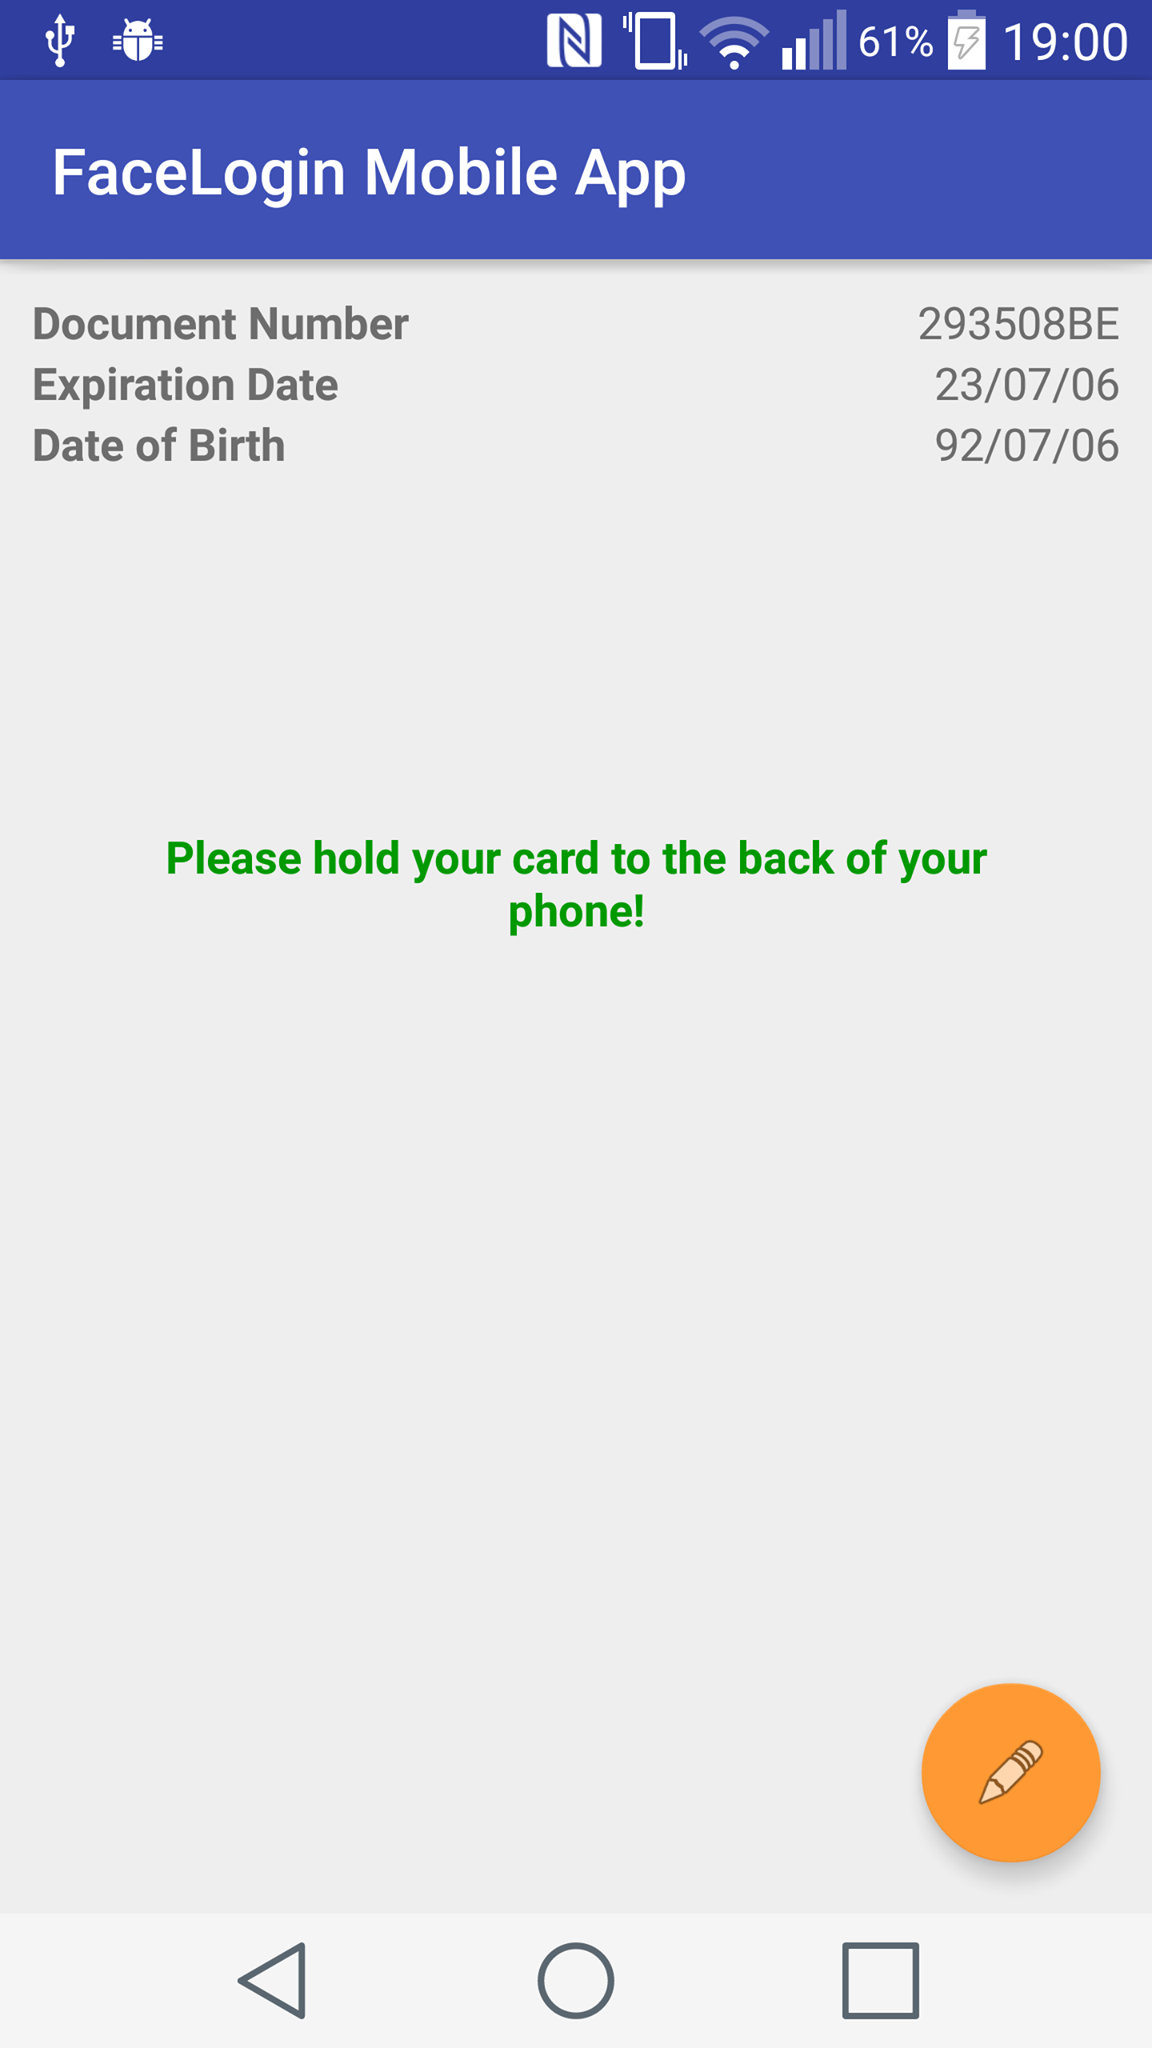
\includegraphics[scale=0.10]{img/app_main_screen}
    \caption{Alkalmazás főoldal}
 \end{minipage}
 \begin{minipage}{.30\textwidth} 
\centering
     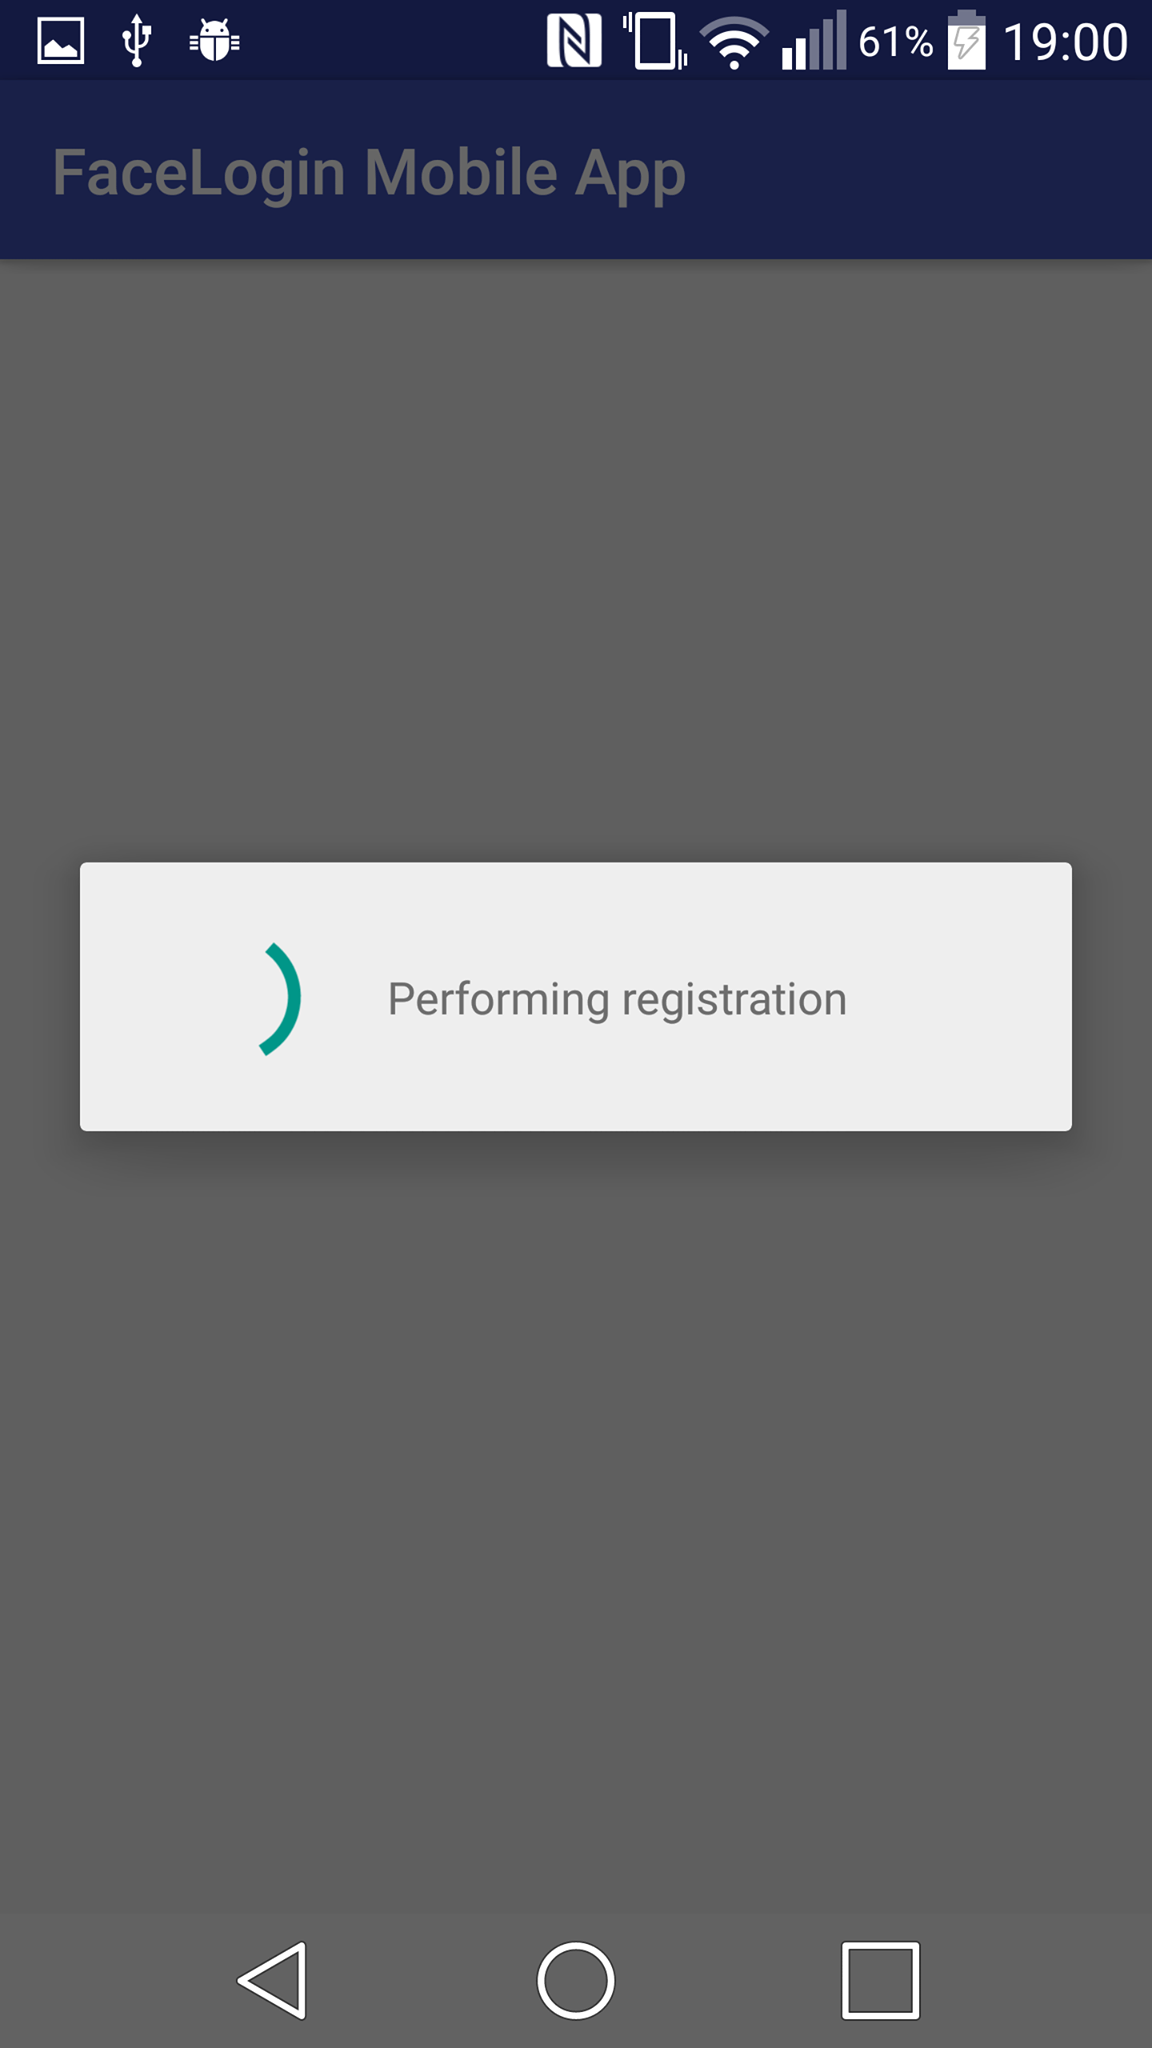
\includegraphics[scale=0.10]{img/performing_registration}
     \caption{Regisztráció folyamatban}
 \end{minipage}
 \begin{minipage}{.30\textwidth} 
\centering
     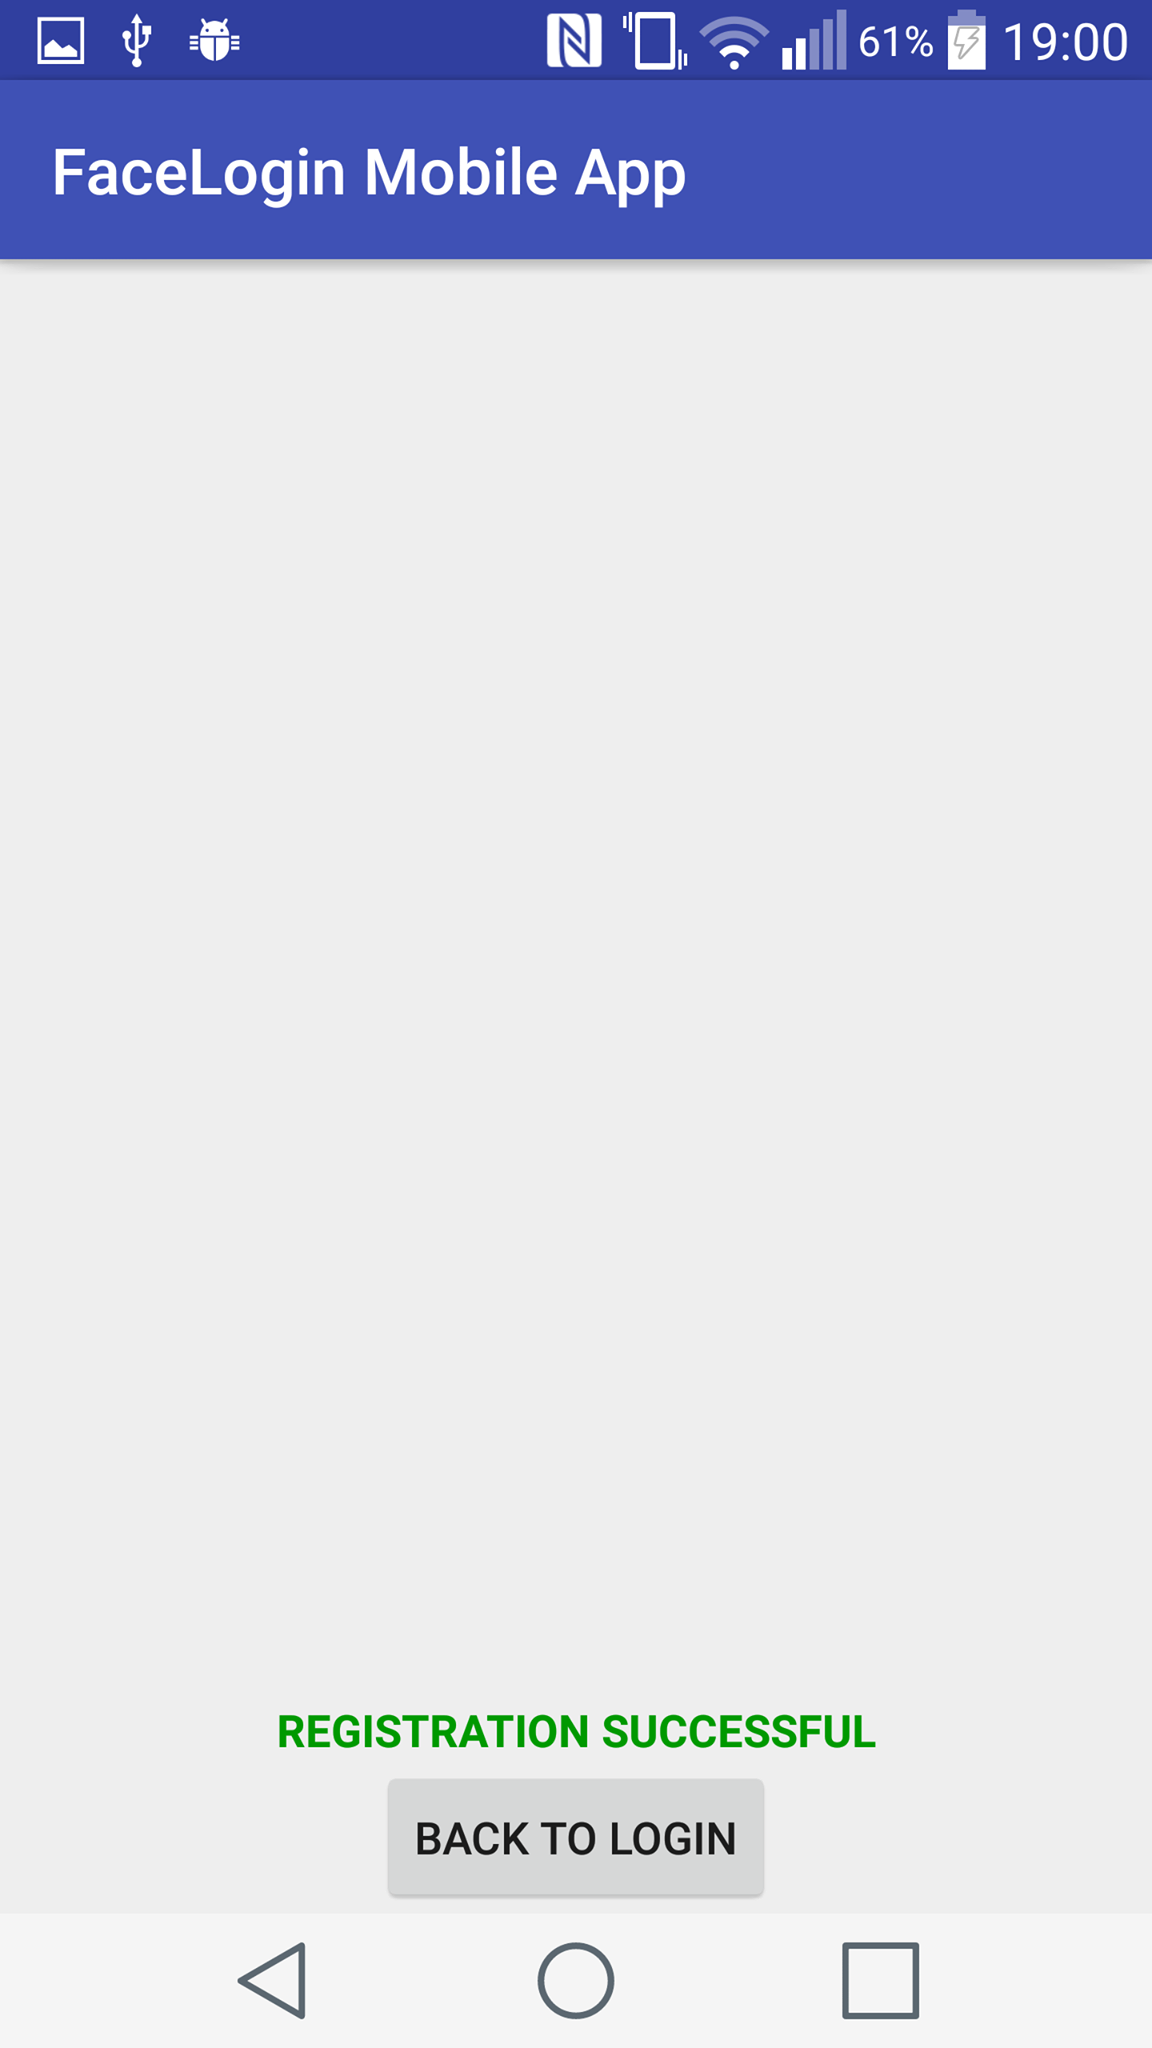
\includegraphics[scale=0.10]{img/registration_successful}
     \caption{Sikeres regisztráció}
 \end{minipage}
\end{figure}
\clearpage
\subsection{Bejelentkezés folyamata}
Sikeres regisztráció után rögtön be lehet jelentkezni az adott weboldalra. Ehhez a főoldalon (19. ábra) a "LOGIN" gombra kell kattintani. Ezután átirányításra kerülünk az IDX szerverre, ahol a megjelenő szövegmezőbe a felhasználónév megadásával folytathatjuk a bejelentkezést. Fontos megjegyezni, hogy egyszer lehet csak próbálkozni a kihívás - válasz nehezebb kijátszása érdekében, így hibás adat megadása esetén a folyamatot elölről kell kezdeni.
\\Létező felhasználónév megadása esetén újabb oldal jelenik meg, ahol először a "Start App" gombra kattintva megnyílik a már regisztrációnál bemutatott alkalmazás.
\\Az alkalmazásból visszatérve a bejelentkezés gombra kattintva folytathatjuk a bejelentkezést. Amennyiben a telefonon történt azonosítás is sikeres volt, továbbításra kerülünk a védett weboldalra. Hiba esetén a főoldalra kerülünk, és a folyamatot elölről kell kezdeni.


\subsection{Bejelentkezés lépései a mobil alkalmazásban}
Amennyiben a fentebb leírt módon minden adat ki van töltve, az NFC be van kapcsolva, úgy a személyi igazolvány telefon hátfalához tartásával folytatódik a bejelentkezés. Első lépésben authentikálja a kártyát a rendszer (27.ábra), majd ellenőrzi, hogy az adott felhasználónévhez tartozó igazolványszám egyezik-e (28. ábra).
\\Amennyiben az első lépés sikeres volt, a kihívás - válasz végrehajtása következik. A képernyőn megjelenik a végrehajtandó kihívás, majd a telefon visszaszámol háromtól. A visszaszámolás végén kell a kért kihívást végrehajtani. Fontos, hogy ne korábban mozgassuk a fejünket, mert akkor az elfogadás sikerességének esélye csökkenhet.
A kihívás teljesítése után felugró ablakban a "performing challenge verification" szöveg olvasható (29. ábra), amíg ez a felirat nem tűnik el, ne lépjünk vissza az alkalmazásban! Miután a szerver kiértékelte a kihívást, a képernyőre kerül kiírásra annak eredménye, ami lehet elfogadott vagy elutasított. Elfogadott kihívás esetén a böngészőben a "Bejelentkezés" gombra kattintva a védett weboldalra jutunk. Elutasítás esetén a bejelentkezést újra kell kezdeni.

\begin{figure}[h]
 \begin{minipage}{.30\textwidth} 
\centering
    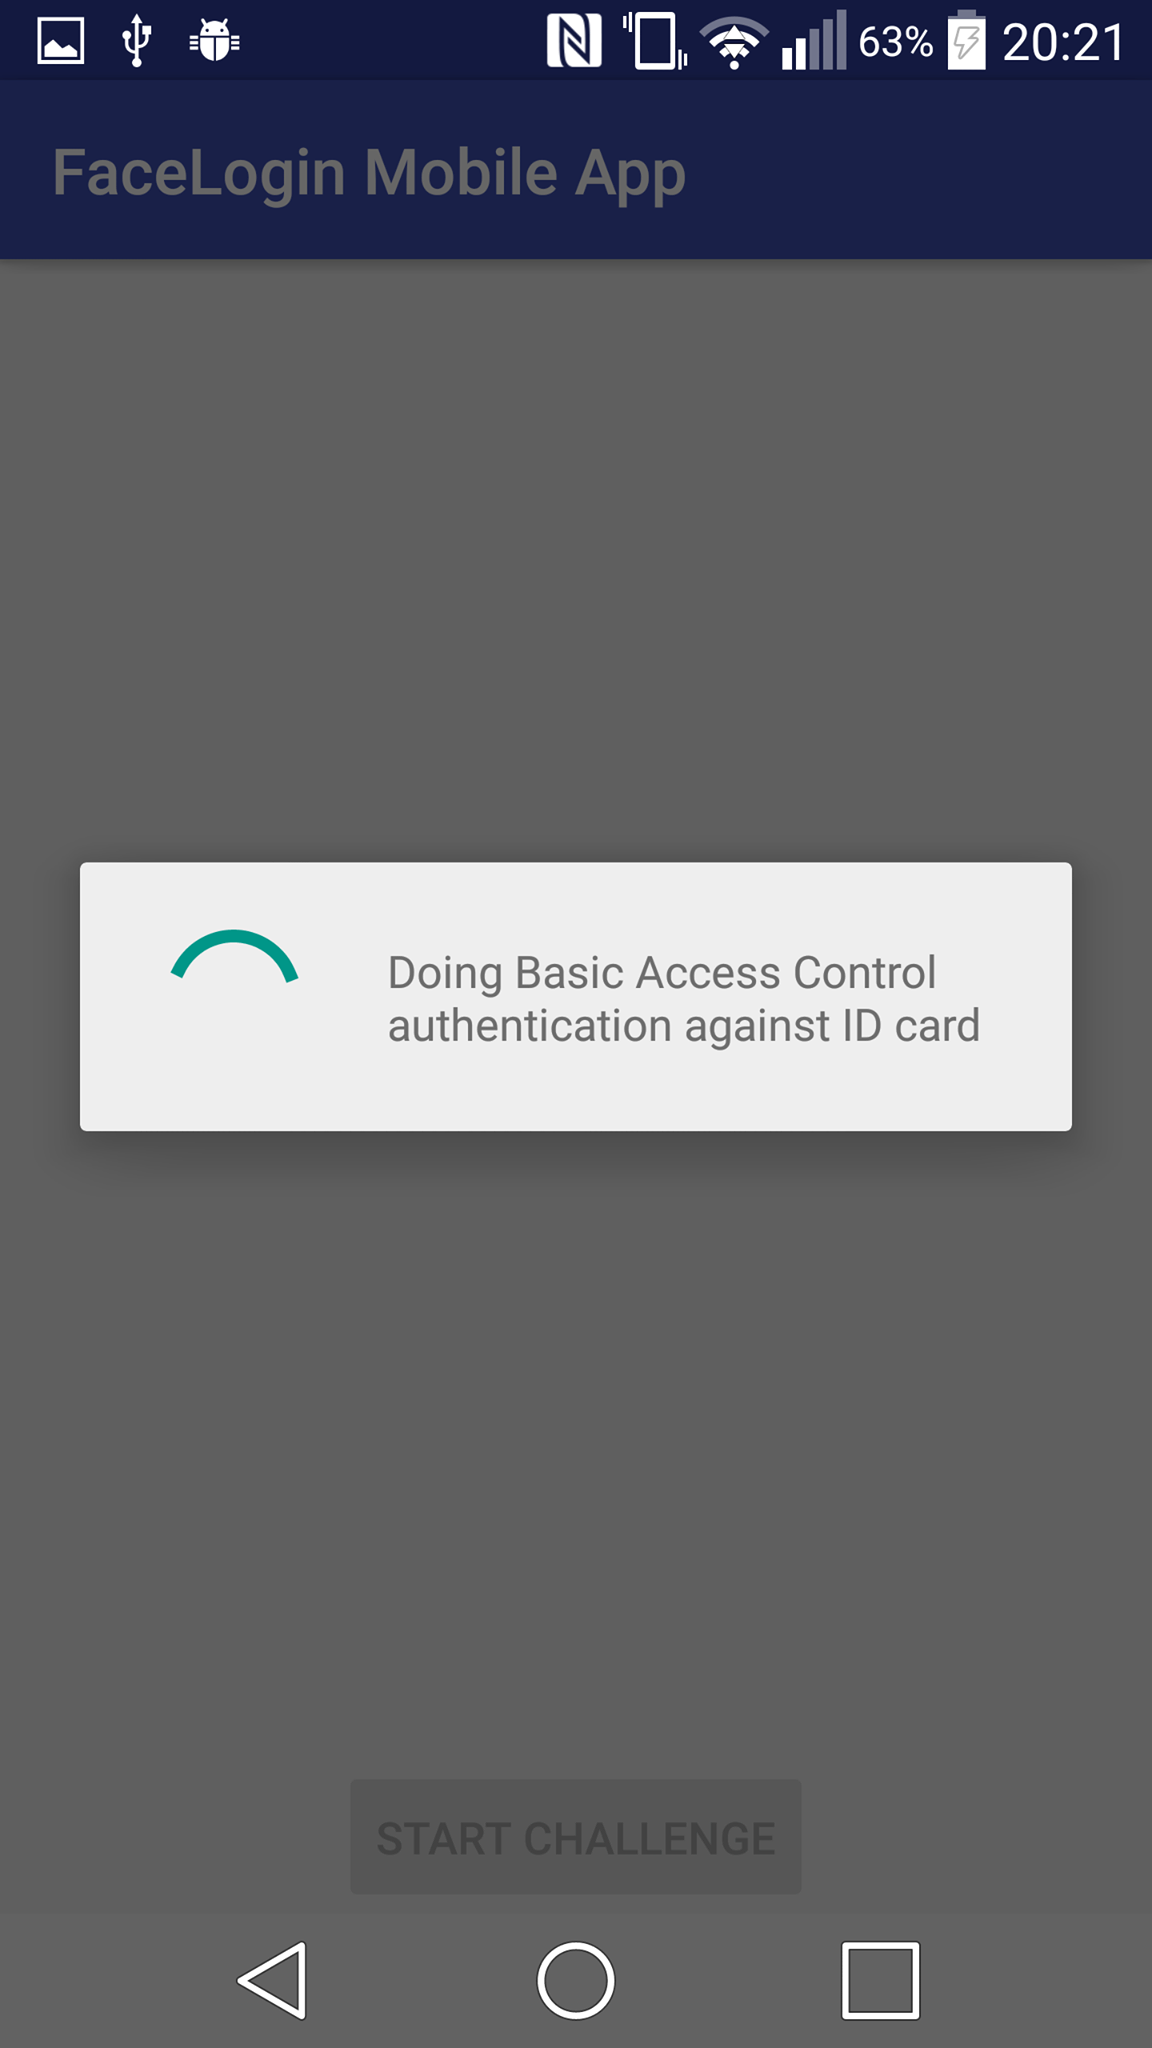
\includegraphics[scale=0.10]{img/BAC}
    \caption{Kártya verifikáció}
 \end{minipage}
 \begin{minipage}{.30\textwidth} 
\centering
     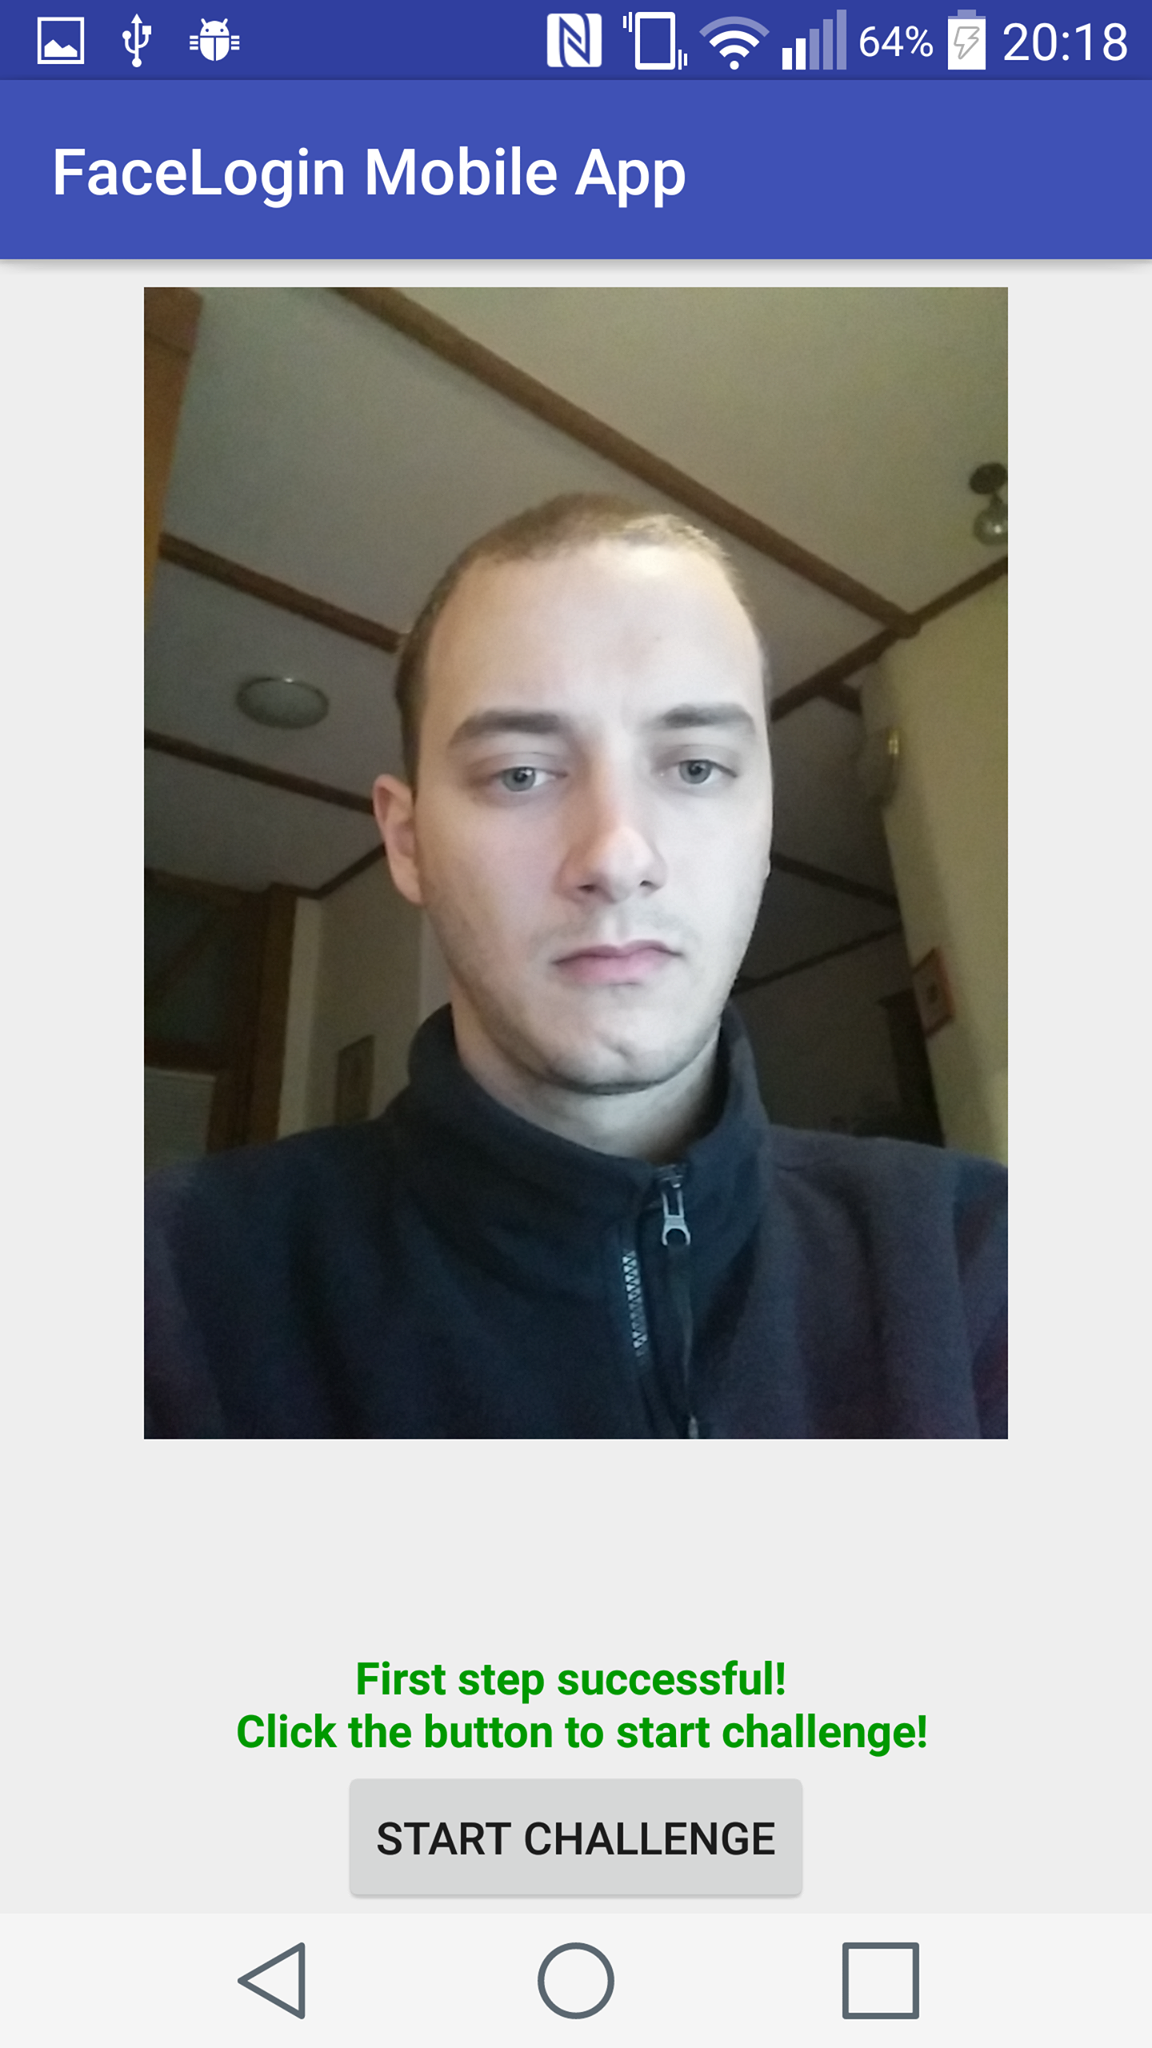
\includegraphics[scale=0.10]{img/first_step_success}
     \caption{Kártya elfogadva, gombnyomásra továbblépés a kihíváshoz}
 \end{minipage}
 \begin{minipage}{.30\textwidth} 
\centering
     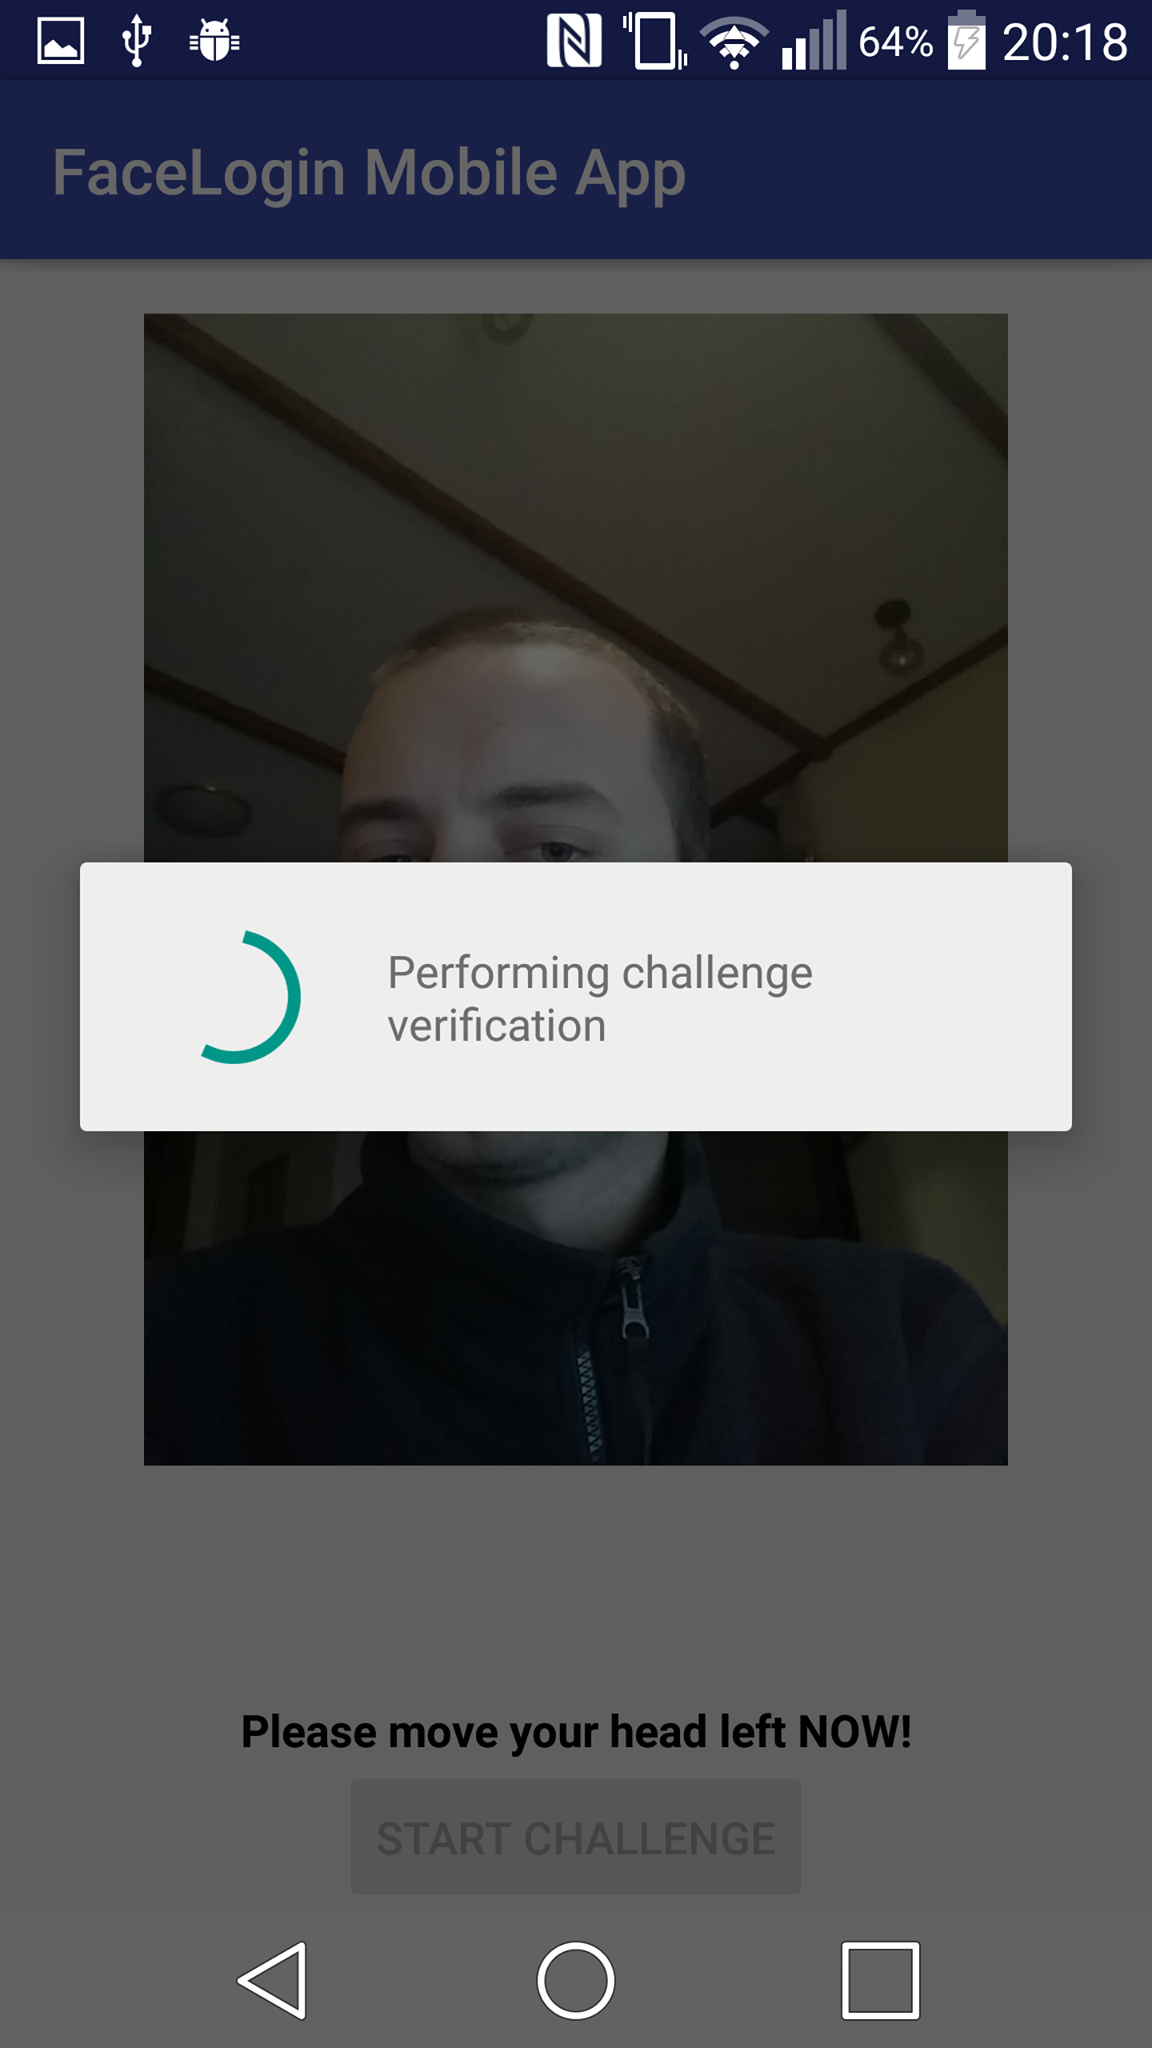
\includegraphics[scale=0.10]{img/performing_challenge_verification}
     \caption{Várakozás a kihívás teljesítésének kiértékelésére}
 \end{minipage}
\end{figure}

\subsection{Bejelentkezés elutasítása}
Sikertelen azonosítás vagy kihívás teljesítés esetén a bejelentkezés elutasításra kerül. Az okok lehetnek:

\begin{itemize}
\item A kártya azonosítása nem sikerült, az alkalmazásban megadott hibás adatok miatt, vagy egyéb kommunikációs probléma miatt (például túl hamar lett eltávolítva a kártya, gyenge volt az NFC jel, stb.) (30. ábra)
\item A megadott kártyaszám nem egyezik a megadott felhasználóhoz tartozó kártyaszámmal (31. ábra)
\item A kihívás nem került elfogadásra (32. ábra). Nem részletezzük, hogy a kihívás melyik része nem sikerült, hogy egy esetleges támadás ne tudja szűkíteni a támadási pontjait.
\end{itemize}

\begin{figure}[h]
 \begin{minipage}{.30\textwidth} 
\centering
    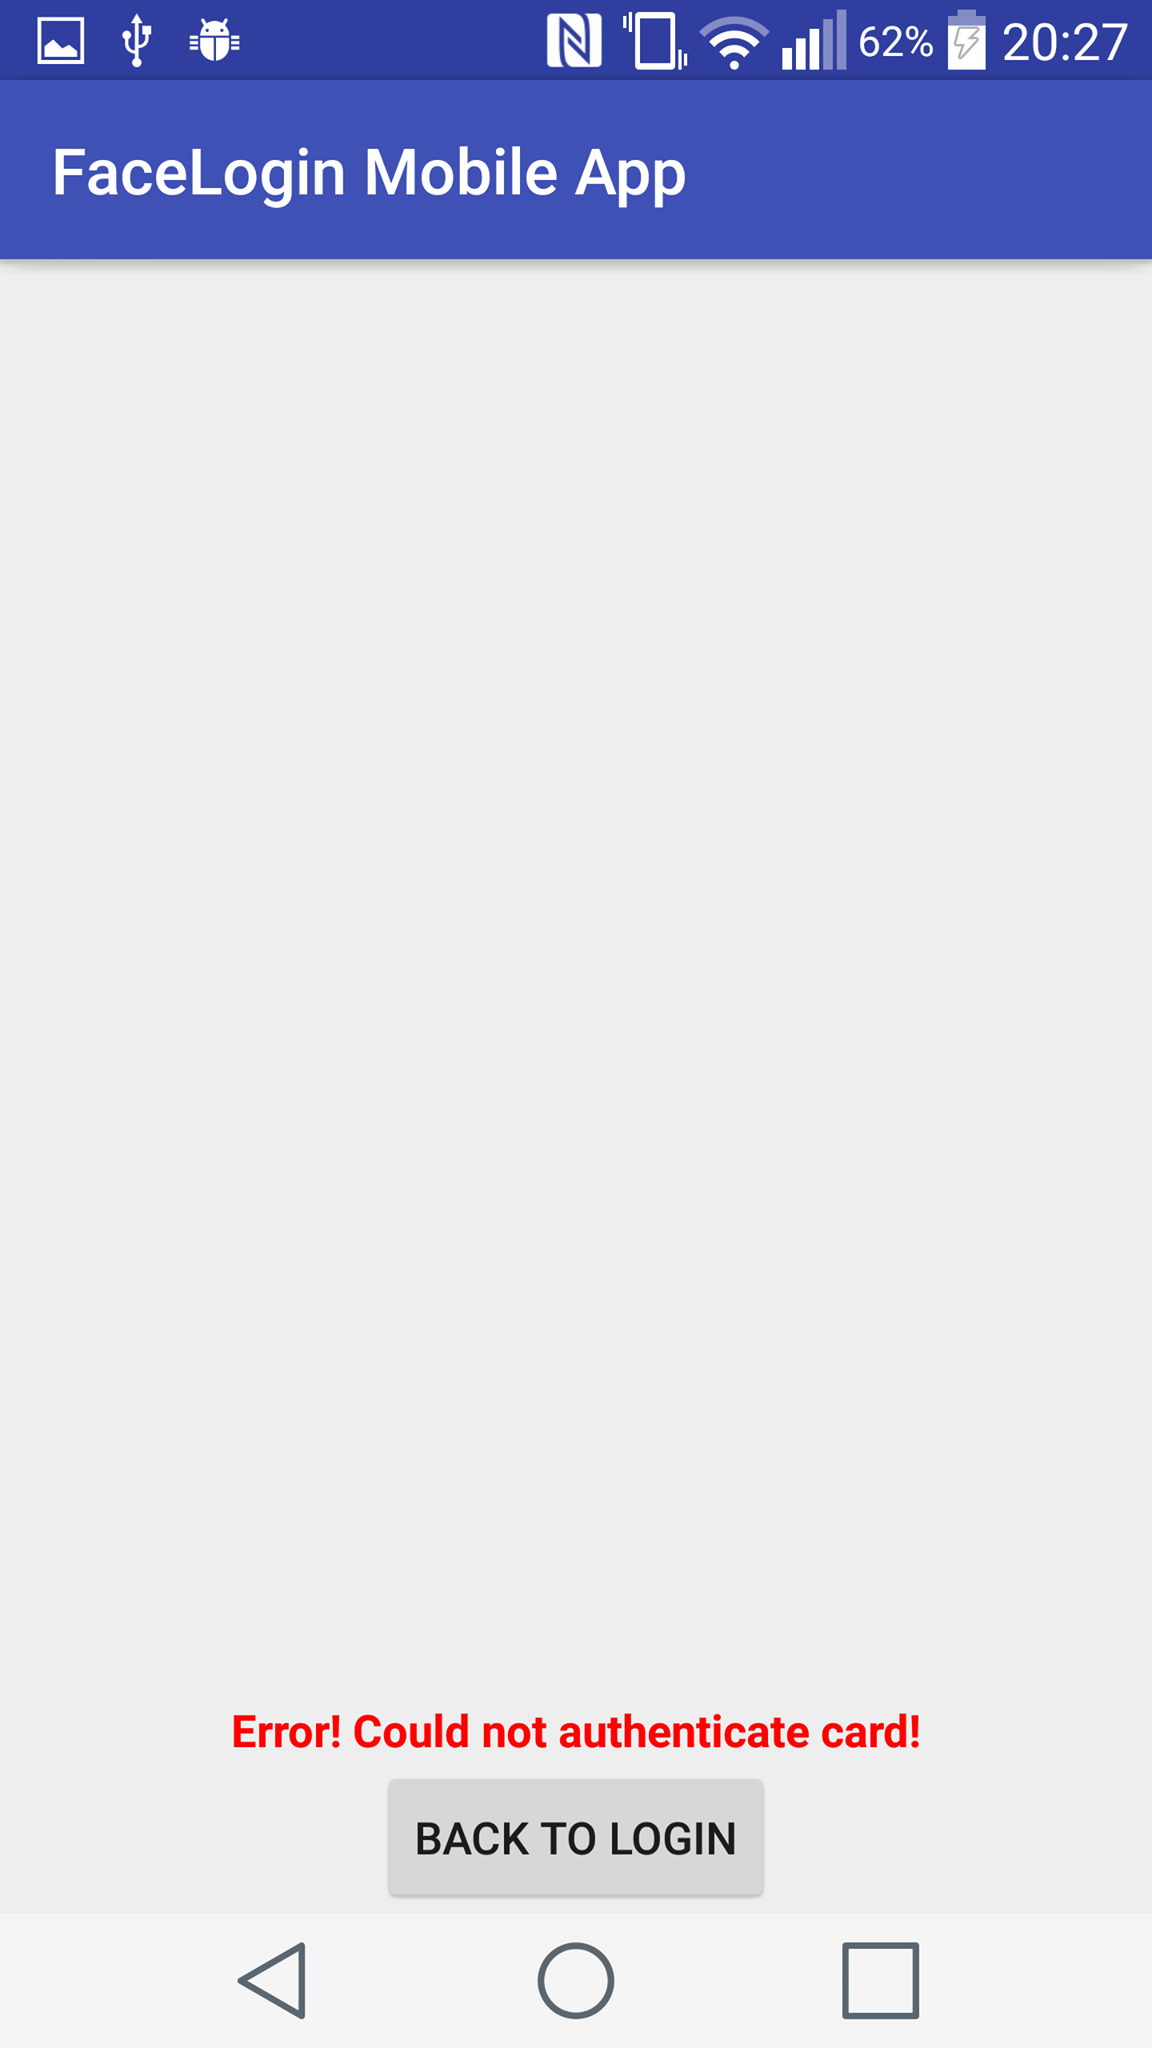
\includegraphics[scale=0.10]{img/card_auth_fail}
    \caption{Kártya azonosítás nem sikerült}
 \end{minipage}
 \begin{minipage}{.30\textwidth} 
\centering
     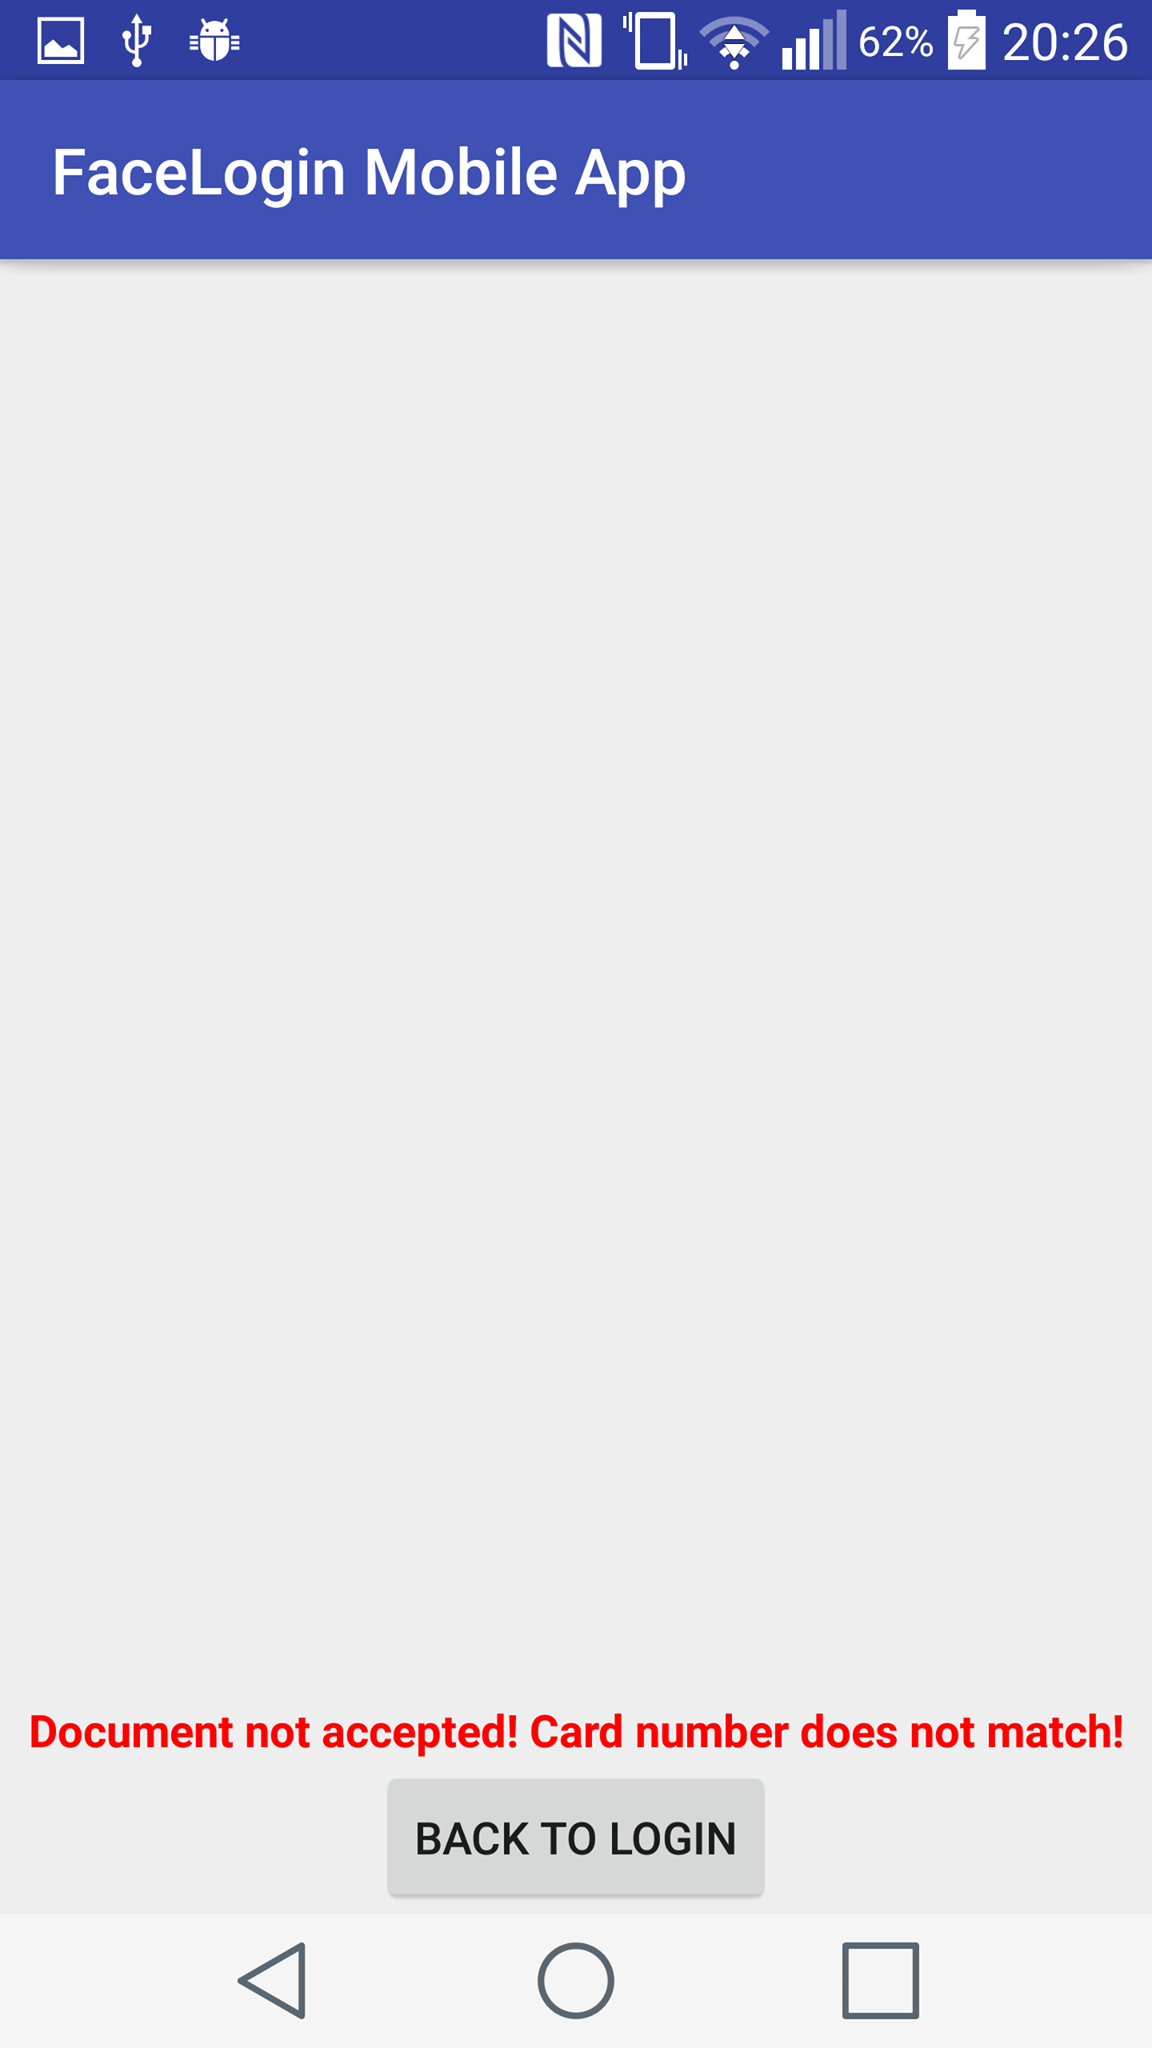
\includegraphics[scale=0.10]{img/card_number_does_not_match}
     \caption{A megadott felhasználóhoz nem ez a kártyaszám tartozik}
 \end{minipage}
 \begin{minipage}{.30\textwidth} 
\centering
     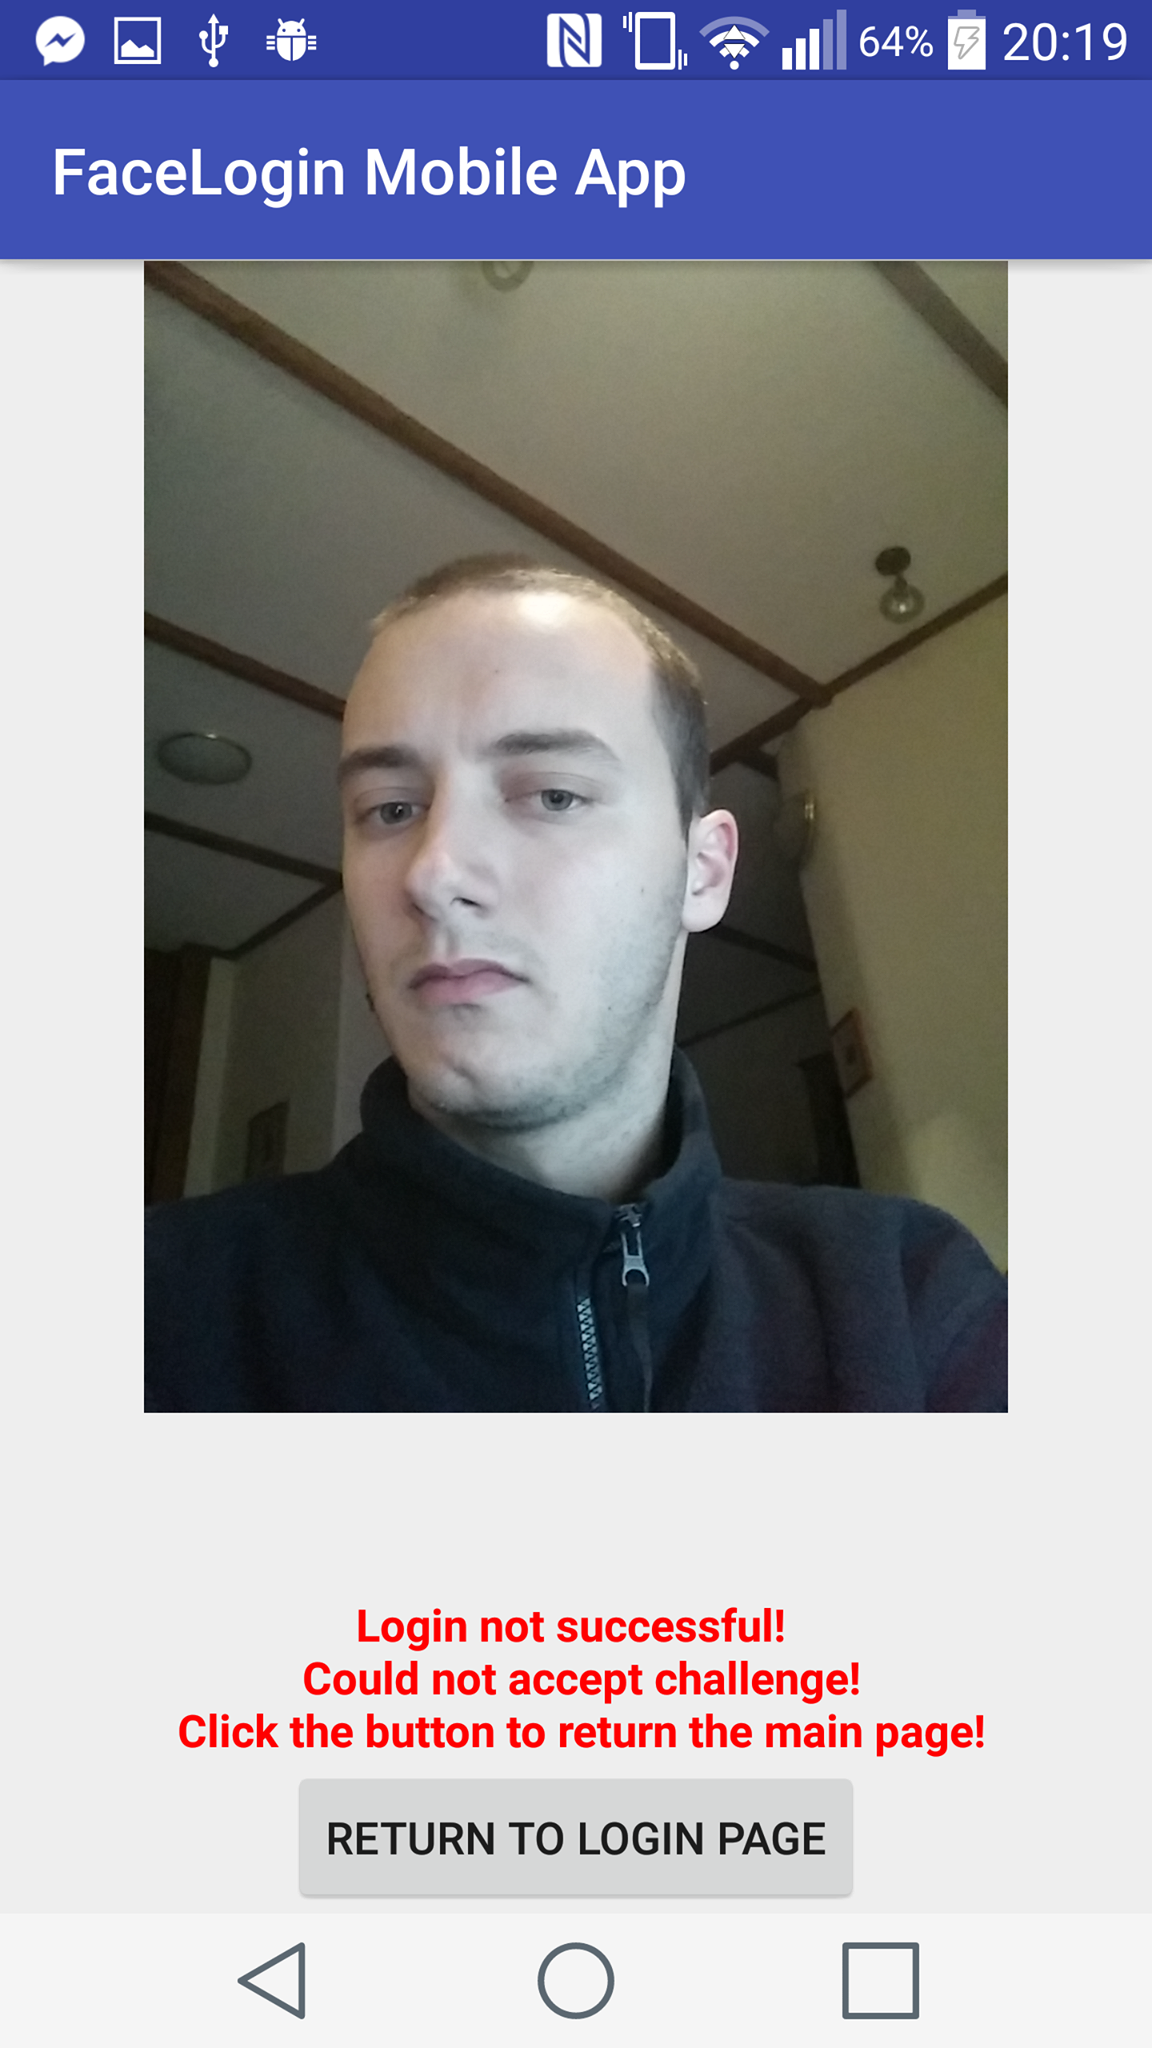
\includegraphics[scale=0.10]{img/could_not_accept_challenge}
     \caption{Kihívásra adott válasz nem volt megfelelő}
 \end{minipage}
\end{figure}
\subsection{Kijelentkezés}
A jelenlegi tesztoldal egyedüli funkciója hogy kiírja a bejelentkezett felhasználó regisztrált felhasználónevét. Kijelentkezés a menüpontban található kijelentkezés gombra kattintva hajtható végre. Ezután a session törlődik, és újból lehet bejelentkezéssel próbálkozni akár ugyanazzal a felhasználóval, akár egy másikkal.

\newpage